\fancyhf{}
\fancyfoot[CO, CE]{ \thepage}

\chapter{Results}
\label{chapter4}

Summary of ASIC Parameters:
\begin{enumerate}
    \item \textbf{Simulation Cycles}:  
  Number of clock cycles required to complete a neural network layer, represented by \( N_{cycles} \)
\item \textbf{Run Time (seconds)}:  
The time taken to simulate the neural network layer, measured in seconds. It is calculated as:
\[
T = \frac{N_{cycles}}{f_{clock}}
\]
\item \textbf{Total Power}:  
The total power consumed by the ASIC during operation, represented by \( P_{total} \), typically measured in watts (W).

\item \textbf{Area}:  
The physical area occupied by the ASIC layout, typically determined after synthesis or place and route steps, measured in square micrometers (\(\mu m^2\)).

\item \textbf{GFLOPS (Giga Floating Point Operations Per Second)}:  
A performance metric representing the number of floating-point operations per second, calculated as:
\[
GFLOPS = \frac{\text{Total Floating Point Operations}}{\text{Execution Time} \times 10^9}
\]

\item \textbf{GFLOPS/W}:  
An efficiency metric representing the number of GFLOPS the ASIC can perform per watt of power consumed:
\[
GFLOPS/W = \frac{GFLOPS}{P_{total}}
\]

\item \textbf{Energy}:  
The total energy consumed during the computation, typically measured in joules (J). It is calculated as:
\[
E = P_{total} \times T
\]
\end{enumerate}

\section{Loop Permutation}
\subsection{Convolution Layer}
Loop permutation for Convolution layer has 2 cases:
\begin{enumerate}
 \item Kernels with no. of input channels 1.
 \item Kernels with no. of input channels $>$ 1.
\end{enumerate}

\subsubsection{Case 1: Kernels with no. of input channels 1.}


\begin{table}[H]
\centering
\caption{AlexNet Convolution layer-1 dimensions}
\label{tab:permConvolutionCase1Dim}
 \begin{tabular}{|c|c|c|c|c|c|c|c|c|c|c|} \hline  
 
 \multirow{2}{*}{\textbf{Layer dimensions}} &  
 \multicolumn{3}{|c|}{\textbf{Input}} &  
 \multicolumn{4}{|c|}{\textbf{Kernel}} &  
 \multicolumn{3}{|c|}{\textbf{Output}}\\ \cline{2-11}
 & H &  W &  C&  H &  W &  C &  F &  H &  W & F\\ \hline  
 \textbf{Actual layer} &  227 &  227 &  3 & 11 & 11 & 3 & 96 & 55 & 55 & 96\\ \hline 
 \textbf{Executed layer} &  227 &  227 &  \cellcolor{yellow}1 & 11 & 11 & 3 & \cellcolor{yellow}1 & 55 & 55 & \cellcolor{yellow}1 \\ \hline 
 \end{tabular}
\end{table}

The Table \ref{tab:permConvolutionCase1Dim} presents the layer information for AlexNet Convolution Layer 1. It shows both the actual configuration of the layer and the configuration used for this experiment. In the actual case, the input is 227×227 with 3 channels, and the kernel is 11×11 with 3 channels and 96 filters, producing an output of 55×55 with 96 filters. After clipping dimensions, the input is reduced to just 1 channel, and the kernel is also simplified to have 1 channel and 1 filter, leading to an output of 55×55 with 1 filter. This modified setup is synthesized to an ASIC.


\begin{table}[H]
\centering
\caption{Output-first permutation}
\label{tab:permConvolutionCase1Op}
\resizebox{\textwidth}{!}{%
 \begin{tabular}{|c|c|c|c|c|c|c|c|}
 \hline
 \textbf{Permutation} & 
 \textbf{Clock cycles}  & 
 \textbf{Total power} & 
 \textbf{Area} & 
 \textbf{Runtime} & 
 \textbf{GFLOPS} & 
 \textbf{GFLOPS/W} & 
 \textbf{Energy} \\ \hline
 0,1,2,3,4,5,6  & 491,687,712 & 0.0078  & 73,324 & 4.9168  & 0.0428 & 5.4414 & 0.0387 \\ \hline
 0,1,2,3,4,6,5  & 491,687,712 & 0.0081  & 76,106 & 4.9168  & 0.0428 & 5.2612 & 0.0400 \\ \hline
 0,1,2,3,5,4,6  & 491,687,712 & 0.0085  & 81,221 & 4.9168  & 0.0428 & 4.9975 & 0.0421  \\ \hline
 0,1,2,3,5,6,4  & 491,687,712 & 0.0085  & 81,203 & 4.9168  & 0.0428 & 5.0033 & 0.0421  \\ \hline
 \end{tabular}
}
\end{table}


The Table \ref{tab:permConvolutionCase1Op} focuses on the results when different loop permutations are applied while processing the output first. Each row represents a different permutation, which determines the order in which loops are executed during the convolution operation. Interestingly, all the permutations in this case result in the same number of clock cycles (491,687,712) and runtime (4.916877 seconds), indicating that the permutations do not affect these metrics. However, there are small variations in total power, area, and energy consumption.
\\

\begin{table}[H]
\centering
\caption{Kernel-first permutation}
\label{tab:permConvolutionCase1Ker}
\resizebox{\textwidth}{!}{%
 \begin{tabular}{|c|c|c|c|c|c|c|c|}
 \hline
 \textbf{Permutation} & 
 \textbf{Clock cycles}  & 
 \textbf{Total power} & 
 \textbf{Area} & 
 \textbf{Runtime} & 
 \textbf{GFLOPS} & 
 \textbf{GFLOPS/W} & 
 \textbf{Energy} \\ \hline
 0,4,5,6,1,2,3 & 595,626,624 & 0.0065 & 55,367  & 5.9562  & 0.0353  & 5.4205 & 0.0388  \\ \hline
 0,4,5,6,1,3,2 & 595,626,624 & 0.0064 & 55,538  & 5.9562  & 0.0353  & 5.5219 & 0.0381  \\ \hline
 0,4,5,6,2,1,3 & 595,626,624 & 0.0065 & 55,763  & 5.9562  & 0.0353  & 5.3711 & 0.0392  \\ \hline
 0,4,5,6,2,3,1 & 595,626,624 & 0.0064 & 56,689  & 5.9562  & 0.0353  & 5.4962 & 0.0383  \\ \hline
 \end{tabular}
}
\end{table}

The Table \ref{tab:permConvolutionCase1Ker} shows the results when different permutations are applied while processing the kernel first. Again, different loop orders are tested, but this time the clock cycles are consistently higher, at 595,626,624, and the runtime is also longer at 5.956266 seconds, compared to the output-first approach. Despite these increases in processing time, total power, area, and energy consumption still show small variations similar to the previous table.

In summary, the key is that loop permutation does not affect the clock cycles or runtime when the input and output channels are both 1, but it does cause slight variations in power, area, and energy consumption. Additionally, the output-first approach is more efficient in terms of clock cycles and runtime compared to the kernel-first approach, which results in higher clock cycles and longer runtimes across all permutations tested.

\subsubsection{Case 2: Kernels with no. of input channels $>$ 1.}

\begin{table}[H]
\centering
\caption{AlexNet Convolution layer-2 dimensions}
\label{tab:permConvolutionCase2Dim}
 \begin{tabular}{|c|c|c|c|c|c|c|c|c|c|c|} \hline  
 
 \multirow{2}{*}{\textbf{Layer dimensions}} &  
 \multicolumn{3}{|c|}{\textbf{Input}} &  
 \multicolumn{4}{|c|}{\textbf{Kernel}} &  
 \multicolumn{3}{|c|}{\textbf{Output}}\\ \cline{2-11}
 & H &  W &  C&  H &  W &  C &  F &  H &  W & F\\ \hline  
 \textbf{Actual layer} &  31 &  31 &  96 & 5 & 5 & 96 & 256 & 27 & 27 & 256\\ \hline 
 \textbf{Executed layer} &  31 &  31 &  \cellcolor{yellow}32 & 5 & 5 & \cellcolor{yellow}32 & \cellcolor{yellow}1 & 27 & 27 & \cellcolor{yellow}1 \\ \hline 
 \end{tabular}
\end{table}

The analysis focuses on the optimization of AlexNet Convolution Layer 2, as shown in Table \ref{tab:permConvolutionCase2Dim}. The actual input dimensions for this layer are 31 (Height) x 31 (Width) x 96 (Channels), while the kernel is 5 (Height) x 5 (Width) x 96 (Channels) x 256 (Filters). The output dimensions are 27 (Height) x 27 (Width) x 256 (Filters). Due to hardware constraints, the actual execution differs, with the input dimensions reduced to 31 x 31 x 32, and the kernel dimensions reduced to 5 x 5 x 32 x 1 for the executed configuration.
\\
\begin{table}[H]
\centering
\caption{First-sweep (kernel permutation)}
\label{tab:permConvolutionCase2Sweep1}
\resizebox{\textwidth}{!}{%
 \begin{tabular}{|c|c|c|c|c|c|c|c|}
 \hline
 \textbf{Permutation} & 
 \textbf{Clock cycles}  & 
 \textbf{Total power} & 
 \textbf{Area} & 
 \textbf{Runtime} & 
 \textbf{GFLOPS} & 
 \textbf{GFLOPS/W} & 
 \textbf{Energy} \\ \hline
 0,1,2,3,4,5,6 & 2,347,358,208 & 0.0132  & 115,534 & 23.4735 & 0.0381  & 2.8910 & 0.3098 \\ \hline
 0,1,2,3,4,6,5 & 1,896,661,248 & 0.0126  & 112,521 & 18.9666 & 0.0472  & 3.7484 & 0.2389 \\ \hline
 0,1,2,3,5,4,6 & 2,347,358,208 & 0.0146  & 127,437 & 23.4735 & 0.0381  & 2.6138 & 0.3427 \\ \hline
 \rowcolor{yellow} 0,1,2,3,5,6,4 & 1,896,661,248 & 0.0126  & 112,424 & 18.9666 & 0.0472  & 3.7484 & 0.2389 \\ \hline
 0,1,2,3,6,4,5 & 1,893,861,888 & 0.0158  & 145,333 & 18.9386 & 0.0473  & 2.9936 & 0.2992 \\ \hline
 0,1,2,3,6,5,4 & 1,893,861,888 & 0.0161  & 146,152 & 18.9386 & 0.0473  & 2.9378 & 0.3049 \\ \hline

 \end{tabular}
}
\end{table}

To find the optimal configuration, a two-step permutation sweep was performed. As shown in Table \ref{tab:permConvolutionCase2Sweep1}, the first sweep focused on finding the best kernel permutation by testing different access patterns for the kernel’s height, width, and channel dimensions. This sweep aimed to minimize clock cycles, power consumption, and energy usage while maximizing GFLOPS (floating-point operations per second) and GFLOPS per watt. After testing several permutations, the kernel permutation 0,1,2,3,5,6,4 emerged as the best configuration, significantly reducing the clock cycles to 1,896,661,248, with lower area (112,424 $\mu\text{m}^2$), total power consumption (0.0126 W) and energy (0.2389 J) compared to the baseline configuration.
\\
\begin{table}[H]
\centering
\caption{Second sweep (output permutation)}
\label{tab:permConvolutionCase2Sweep2}
\resizebox{\textwidth}{!}{%
 \begin{tabular}{|c|c|c|c|c|c|c|c|}
 \hline
 \textbf{Permutation} & 
 \textbf{Clock cycles}  & 
 \textbf{Total power} & 
 \textbf{Area} & 
 \textbf{Runtime} & 
 \textbf{GFLOPS} & 
 \textbf{GFLOPS/W} & 
 \textbf{Energy} \\ \hline
  0,1,2,3,5,6,4  & 1,896,661,248  & 0.0126 & 112,424  & 18.9666  & 0.0472  & 3.7484 & 0.2389  \\ \hline
  0,1,3,2,5,6,4  & 1,896,661,248  & 0.0126 & 112,879  & 18.9666  & 0.0472  & 3.7484 & 0.2389  \\ \hline
  \rowcolor{yellow} 0,2,1,3,5,6,4  & 1,896,661,248  & 0.0125 & 111,997  & 18.9666  & 0.0472  & 3.7784 & 0.2370  \\ \hline
  0,2,3,1,5,6,4  & 1,896,661,248  & 0.0125 & 112,055  & 18.9666  & 0.0472  & 3.7784 & 0.2370  \\ \hline
  0,3,1,2,5,6,4  & 1,896,661,248  & 0.0127 & 112,793  & 18.9666  & 0.0472  & 3.7188 & 0.2408  \\ \hline
  0,3,2,1,5,6,4  & 1,896,661,248  & 0.0125 & 112,054  & 18.9666  & 0.0472  & 3.7784 & 0.2370  \\ \hline

 \end{tabular}
}
\end{table}

Once the optimal kernel permutation was identified, the second sweep targeted the output permutation. Different output access patterns were tested to further refine the configuration. The best output permutation was found to be '0,2,1,3,5,6,4', resulting in even better performance. This permutation reduced the area to 111,997 $\mu\text{m}^2$, total power to 0.0125 W, and energy to 0.2370 J, solidifying it as the most optimal overall permutation.
\\
\begin{table}[H]
\centering
\caption{Loop permutation results}
\label{tab:permConvolutionCase2Results}
\resizebox{\textwidth}{!}{%
 \begin{tabular}{|c|c|c|c|c|c|c|c|}
 \hline
 \textbf{Permutation} & 
 \textbf{Clock cycles}  & 
 \textbf{Total power} & 
 \textbf{Area} & 
 \textbf{Runtime} & 
 \textbf{GFLOPS} & 
 \textbf{GFLOPS/W} & 
 \textbf{Energy} \\ \hline
 Baseline permutation& 2,347,358,208 & 0.0132  & 115,534 & 23.4735 & 0.0381  & 2.8910 & 0.3098 \\ \hline
 Best Output-first permutation & 1,896,661,248  & 0.0125 & 111,997  & 18.9666  & 0.0472  & 3.7784 & 0.2370  \\ \hline
 Best Kernel-first permutation & 2,357,954,304 & 0.0133  & 114,968  & 23.5795  & 0.0379 & 2.8563 & 0.3136 \\ \hline

 \end{tabular}
}
\end{table}

In this comparison presented in the Table \ref{tab:permConvolutionCase2Results}, the best output-first permutation clearly outperforms both the baseline and the best kernel-first permutation in terms of clock cycles. The baseline registers 2,347,358,208 clock cycles, whereas the best output-first permutation achieves a significant reduction to 1,896,661,248. The best kernel-first permutation, although an improvement over the baseline, still has a higher clock cycle count at 2,357,954,304, highlighting the superior performance of the output-first approach.

When it comes to total power consumption, the best output-first permutation is the most efficient, consuming 0.0125 W, which is lower than both the baseline's 0.0132 W and the best kernel-first permutation's 0.0133 W. This lower power consumption contributes to the overall efficiency of the output-first strategy. Additionally, the best output-first permutation requires the least area at 111,997 $\mu\text{m}^2$, followed by the best kernel-first permutation at 114,968 $\mu\text{m}^2$, and the baseline, which uses 115,534 $\mu\text{m}^2$.

In terms of runtime, the best output-first permutation shows a substantial reduction with 18.9666 seconds, compared to the baseline's 23.4735 seconds and the best kernel-first permutation's 23.5795 seconds. This reflects the ability of the output-first permutation to complete computations faster. Similarly, the best output-first permutation achieves the highest GFLOPS at 0.0472, significantly better than both the baseline's 0.0381 and the best kernel-first permutation's 0.0379.

For GFLOPS/W, the best output-first permutation again excels with 3.7784, while the baseline offers 2.8910, and the best kernel-first permutation falls slightly behind with 2.8563. This demonstrates that the output-first permutation is not only faster but also more energy-efficient. Finally, in terms of energy consumption, the best output-first permutation consumes the least energy at 0.2370, far outperforming the baseline's 0.3098 and the best kernel-first permutation's 0.3136.

In summary, the best output-first permutation provides the best overall performance across all parameters, showing superior efficiency in terms of clock cycles, power consumption, runtime, GFLOPS, GFLOPS/W, and energy usage. The best kernel-first permutation offers some improvements over the baseline, but it does not match the efficiency gains seen with the output-first approach.

\subsection{Depth-wise Convolution Layer}


Loop permutation for Depth-wise Convolution layer has 2 cases:
\begin{enumerate}
 \item Case 1 : Kernels with no. of input channels 1.
 \item Case 2 : Kernels with no. of input channels $>$ 1.
\end{enumerate}


\subsubsection{Case 1: Kernels with number of input channels 1.}


\begin{table}[H]
\centering
\caption{Mobilenet-v3-small Depth-wise Convolution Layer 1:}
\label{tab:permDConvolutionCase1Dim}
 \begin{tabular}{|c|c|c|c|c|c|c|c|c|c|c|} \hline  
 
 \multirow{2}{*}{\textbf{Layer dimensions}} &  
 \multicolumn{3}{|c|}{\textbf{Input}} &  
 \multicolumn{3}{|c|}{\textbf{Kernel}} &  
 \multicolumn{3}{|c|}{\textbf{Output}}\\ \cline{2-10}
 & H &  W &  C&  H &  W &  C &  H &  W & F\\ \hline  
 \textbf{Actual layer} &  113 &  113 & 16 & 3 & 3 & 16 & 56 & 56 & 16\\ \hline 
 \textbf{Executed layer} &  113 &  113 &  \cellcolor{yellow}1 & 3 & 3 & \cellcolor{yellow}1 & 56 & 56 & \cellcolor{yellow}1 \\ \hline 
 \end{tabular}
\end{table}

In this example, the first Depth-wise Convolutional (Depth-wise Convolution) layer of the MobileNet-V3-Small architecture is analyzed. The original input dimensions are 113 (Height) x 113 (Width) x 16 (Channel), with a kernel size of 3 (Height) x 3 (Width) x 16 (Channel), producing an output of 56 (Height) x 56 (Width) x 16 (channel). However, after applying dimensional clipping, the number of input channels is reduced to 1, as shown in Table \ref{tab:permDConvolutionCase1Dim}.

\begin{table}[H]
\centering
\caption{Output-first permutation}
\label{tab:permDConvolutionCase1Op}
\resizebox{\textwidth}{!}{%
 \begin{tabular}{|c|c|c|c|c|c|c|c|}
 \hline
 \textbf{Permutation} & 
 \textbf{Clock cycles}  & 
 \textbf{Total power} & 
 \textbf{Area} & 
 \textbf{Runtime} & 
 \textbf{GFLOPS} & 
 \textbf{GFLOPS/W} & 
 \textbf{Energy} \\ \hline
  0,1,2,3,4,5  & 2,679,904 & 0.0076  & 62,864 & 0.0267 & 0.0337 & 4.4344 & 0.000204 \\ \hline
  0,1,2,3,5,4  & 2,679,904 & 0.0074 & 61,432 & 0.0267 & 0.0337 & 4.4995 & 0.000201 \\ \hline
  0,1,3,2,4,5  & 2,679,904 & 0.0075 & 61,880 & 0.0267 & 0.0337 & 4.4579 & 0.000203 \\ \hline
  0,1,3,2,5,4  & 2,679,904 & 0.0074 & 61,432 & 0.0267 & 0.0337 & 4.4995 & 0.000201 \\ \hline

 \end{tabular}
}
\end{table}

In the Table \ref{tab:permDConvolutionCase1Op}, several output-first permutations were explored, but there is no significant difference in performance across the configurations. The clock cycles consistently remain at 2,679,904 for all the permutations. Other performance metrics such as runtime and efficiency also show no substantial variation, confirming that changing the output loop order does not impact the performance for this layer.
\\
\begin{table}[H]
\centering
\caption{Kernel-first permutation}
\label{tab:permDnnCase1Ker}
\resizebox{\textwidth}{!}{%
 \begin{tabular}{|c|c|c|c|c|c|c|c|}
 \hline
 \textbf{Permutation} & 
 \textbf{Clock cycles}  & 
 \textbf{Total power} & 
 \textbf{Area} & 
 \textbf{Runtime} & 
 \textbf{GFLOPS} & 
 \textbf{GFLOPS/W} & 
 \textbf{Energy} \\ \hline
 0,3,4,5,1,2 & 3,953,600 & 0.0070  & 59,034  & 0.0395 & 0.0228 & 3.2311 & 0.000280 \\ \hline
0,3,4,5,2,1 & 3,953,600 & 0.0069  & 57,731  & 0.0395 & 0.0228 & 3.3011 & 0.000274 \\ \hline
0,3,5,4,1,2 & 3,941,824 & 0.0070  & 58,135  & 0.0394 & 0.0229 & 3.2454 & 0.000278 \\ \hline
0,3,5,3,2,1 & 3,941,824 & 0.0069  & 58,023  & 0.0394 & 0.0229 & 3.2920 & 0.000274 \\ \hline

 \end{tabular}
}
\end{table}

Table \ref{tab:permDnnCase1Ker} presents the results for various kernel-first permutations. Similar to the output-first cases, there is no notable change in performance. The clock cycles for these permutations remain at either 3,941,824 or 3,953,600, indicating that kernel-first permutations also have no effect on the overall performance of the depthwise convolutional layer in this scenario.

In summary, the comparison of output-first and kernel-first permutations for the first Depth-wise Convolution layer of MobileNet-V3-Small shows no significant performance differences. The output-first permutations consistently result in 2,679,904 clock cycles, while the kernel-first permutations are slightly higher at 3,941,824 or 3,953,600. Despite this small difference in clock cycles, other performance metrics remain unaffected, indicating that loop permutation has minimal impact on depthwise convolutional layers with single input and output channels.

\subsubsection{Case 2: Kernels with no. of input channels $>$ 1.}

\begin{table}[H]
\centering
\caption{Mobilenet-v3-small Depth-wise Convolution layer 2:}
\label{tab:permDConvolutionCase2Dim}
 \begin{tabular}{|c|c|c|c|c|c|c|c|c|c|c|} \hline  
 
 \multirow{2}{*}{\textbf{Layer dimensions}} &  
 \multicolumn{3}{|c|}{\textbf{Input}} &  
 \multicolumn{3}{|c|}{\textbf{Kernel}} &  
 \multicolumn{3}{|c|}{\textbf{Output}}\\ \cline{2-10}
 & H &  W &  C&  H &  W &  C &  H &  W & F\\ \hline  
 \textbf{Actual layer} &  57 &  57 & 72 & 3 & 3 & 72 & 28 & 28 & 72\\ \hline 
 \textbf{Executed layer} &  57 &  57 &  \cellcolor{yellow}8 & 3 & 3 & \cellcolor{yellow}8 & 28 & 28 & \cellcolor{yellow}8 \\ \hline 
 \end{tabular}
\end{table}

In the Table \ref{tab:permDConvolutionCase2Dim}, the focus is on the input, kernel, and output dimensions of the second Depth-wise Convolution layer in the MobileNet-V3-Small architecture. The actual layer dimensions include an input of 57 x 57 x 72, a kernel of 3 x 3 x 72, and an output of 28 x 28 x 72. However, after dimensional clipping for hardware execution, the executed layer has the number of channels reduced to 8 for both the input and kernel, as well as 8 output filters. 
\\
\begin{table}[H]
\centering
\caption{Sweep (kernel permutation)}
\label{tab:permDConvolutionCase2Sweep}
\resizebox{\textwidth}{!}{%
 \begin{tabular}{|c|c|c|c|c|c|c|c|}
 \hline
 \textbf{Permutation} & 
 \textbf{Clock cycles}  & 
 \textbf{Total power} & 
 \textbf{Area} & 
 \textbf{Runtime} & 
 \textbf{GFLOPS} & 
 \textbf{GFLOPS/W} & 
 \textbf{Energy} \\ \hline
0,3,1,2,4,5 & 3,953,600 & 0.0070  & 59,034  & 0.0395 & 0.0228 & 3.2311 & 0.000280 \\ \hline
0,3,1,2,5,4 & 3,953,600 & 0.0069  & 57,731  & 0.0395 & 0.0228 & 3.3011 & 0.000274 \\ \hline
0,3,2,1,4,5 & 3,941,824 & 0.0070  & 58,135  & 0.0394 & 0.0229 & 3.2454 & 0.000278 \\ \hline
\rowcolor{yellow}0,3,2,1,5,4 & 3,941,824 & 0.0069  & 58,023  & 0.0394 & 0.0229 & 3.2920 & 0.000274 \\ \hline

 \end{tabular}
}
\end{table}

The table \ref{tab:permDConvolutionCase2Sweep} explores the results of a kernel permutation sweep, evaluating the performance of different kernel access patterns. Among the tested permutations, 0,3,2,1,5,4 emerges as the most efficient, achieving the lowest clock cycles of 3,941,824.

\begin{table}[H]
\centering
\caption{Loop permutation results}
\label{tab:permDConvolutionCase2Results}
\resizebox{\textwidth}{!}{%
 \begin{tabular}{|c|c|c|c|c|c|c|c|}
 \hline
 \textbf{Permutation} & 
 \textbf{Clock cycles}  & 
 \textbf{Total power} & 
 \textbf{Area} & 
 \textbf{Runtime} & 
 \textbf{GFLOPS} & 
 \textbf{GFLOPS/W} & 
 \textbf{Energy} \\ \hline
 Baseline permutation & 2,679,904 & 0.0076 & 62,864 & 0.0267 & 0.0337 & 4.4344 & 0.000204 \\ \hline
 Best Output-first permutation  & 2,379,933 & 0.0123   & 101,655 & 0.0237 & 0.0426 & 3.4710 & 0.000293 \\ \hline
Best Kernel-first permutation:  & 3,808,440 & 0.0112   & 94,712  & 0.0380 & 0.0266 & 2.3821 & 0.000427 \\ \hline
 \end{tabular}
}
\end{table}

The Table \ref{tab:permDConvolutionCase2Results} compares the performance metrics for the baseline, best output-first, and best kernel-first permutations. In terms of clock cycles, the baseline permutation stands at 2,679,904, whereas the best output-first permutation improves this, reducing the clock cycles to 2,379,933. However, the best kernel-first permutation performs worse, with 3,808,440 clock cycles.

For total power, the baseline consumes 0.0076 W, while the best output-first permutation slightly lowers this to 0.0123 W. The best kernel-first permutation, however, has the highest power consumption at 0.0124 W. The area required by each permutation shows minimal variation, with the baseline requiring 62,864, $\mu\text{m}^2$ the best output-first needing 61,055 $\mu\text{m}^2$, and the best kernel-first taking up 94,712 $\mu\text{m}^2$. The runtime also follows a similar trend, with the baseline at 0.0267 seconds, the output-first at 0.0237 seconds, and the kernel-first considerably higher at 0.0380 seconds.

In terms of GFLOPS, the output-first permutation achieves the highest value at 0.0456, outperforming both the baseline (0.0337) and kernel-first (0.03204). Similarly, GFLOPS/W is highest for the output-first permutation at 3.8004, compared to the baseline’s 4.4344 and the kernel-first permutation’s lower efficiency at 2.821.

Lastly, regarding energy consumption, the output-first permutation again proves to be the most efficient at 0.000191, lower than both the baseline’s 0.000204 and the kernel-first’s higher energy consumption of 0.000247. This comparison highlights that the best output-first permutation consistently outperforms both the baseline and the kernel-first permutation across almost all parameters, making it the most efficient configuration overall.

\subsection{Fully Connected (FC) Layer}

Loop permutation for FC layer has 2 cases:
\begin{enumerate}
 \item Small layer.
 \item Large layer.
\end{enumerate}

\subsubsection{Case 1: Small layer.}

\begin{table}[H]
\centering
\caption{LeNet Fully Connected (FC) layer 2:}
\label{tab:permFcCase1Dim}
 \begin{tabular}{|c|c|c|c|c|c|c|c|c|c|c|} \hline  
 
 \multirow{2}{*}{\textbf{Layer dimensions}} &  
 \multicolumn{2}{|c|}{\textbf{Input}} &  
 \multicolumn{2}{|c|}{\textbf{Weights}} &  
 \multicolumn{2}{|c|}{\textbf{Output}}\\ \cline{2-7}
 & H &  W &  H &  W & H &  W\\ \hline  
 \textbf{Actual layer} &  1 &  84 & 84 & 10 & 1 & 10 \\ \hline 
 \textbf{Executed layer} &  1 &  84 & 84 & 10 & 1 & 10 \\ \hline 
 \end{tabular}
\end{table}

In Table \ref{tab:permFcCase1Dim}, the dimensions for the second fully connected (FC) layer in the LeNet architecture are presented. The input is 1 x 84, the weights are 84 x 10, and the output is 1 x 10 for the actual layer. These dimensions remain unchanged during execution, meaning no dimensional reduction or clipping was applied.
\\
\begin{table}[H]
\centering
\caption{Loop permutation sweep}
\label{tab:permFcCase1Sweep}
\resizebox{\textwidth}{!}{%
 \begin{tabular}{|c|c|c|c|c|c|c|c|}
 \hline
 \textbf{Permutation} & 
 \textbf{Clock cycles}  & 
 \textbf{Total power} & 
 \textbf{Area} & 
 \textbf{Runtime} & 
 \textbf{GFLOPS} & 
 \textbf{GFLOPS/W} & 
 \textbf{Energy} \\ \hline
0,1,2,3  & 7,652   & 0.0060 & 52,803 & 7.7e-05  & 0.0218 & 3.6302 & 4.6277e-07 \\ \hline
\rowcolor{yellow} 0,1,3,2  & 4,706   & 0.0065 & 61,364 & 4.7e-05  & 0.0357 & 5.4241 & 3.0973e-07 \\ \hline
0,2,1,3  & 7,652   & 0.0059 & 52,454 & 7.7e-05  & 0.0218 & 3.6668 & 4.5815e-07 \\ \hline
0,2,3,1  & 7,652   & 0.0059 & 52,441 & 7.7e-05  & 0.0218 & 3.6668 & 4.5815e-07 \\ \hline
0,3,1,2  & 4,706   & 0.0066 & 61,975 & 4.7e-05  & 0.0357 & 5.4077 & 3.1067e-07 \\ \hline
0,3,2,1  & 4,706   & 0.0065 & 61,931 & 4.7e-05  & 0.0357 & 5.4241 & 3.0973e-07 \\ \hline
 \end{tabular}
}
\end{table}

In Table \ref{tab:permFcCase1Dim}, a loop permutation sweep was conducted to evaluate the performance across different permutations. The baseline configuration (0,1,2,3) results in 7,652 clock cycles and a runtime of 7.7e-05 seconds. The baseline also records a GFLOPS of 0.0218, GFLOPS/W of 3.6302, and consumes 0.0060 W total power. The area required for the baseline configuration is 52,803 $\mu\text{m}^2$, and the energy consumption is 4.6277e-07 J.

When compared to the baseline, the 0,1,3,2 permutation shows a significant improvement in multiple aspects. It reduces the clock cycles to 4,706, greatly enhancing processing speed. It also improves GFLOPS to 0.0357 and GFLOPS/W to 5.4241, reflecting better computational efficiency. While the total power consumption increases slightly to 0.0065 W, the area required increases to 61,364 $\mu\text{m}^2$, which is higher than the baseline. Despite this larger area, the energy consumption is notably reduced to 3.0973e-07 J, making this permutation more energy-efficient. Thus, even though the (0,1,3,2) permutation requires more area, it delivers much better performance in terms of speed and energy efficiency compared to the baseline.

\subsubsection{Case 2: Large layer.}

\begin{table}[H]
\centering
\caption{AlexNet Fully Connected (FC) layer 1:}
\label{tab:permFcCase2Dim}
 \begin{tabular}{|c|c|c|c|c|c|c|c|c|c|c|} \hline  
 
 \multirow{2}{*}{\textbf{Layer dimensions}} &  
 \multicolumn{2}{|c|}{\textbf{Input}} &  
 \multicolumn{2}{|c|}{\textbf{Weights}} &  
 \multicolumn{2}{|c|}{\textbf{Output}}\\ \cline{2-7}
 & H &  W &  H &  W & H &  W\\ \hline  
 \textbf{Actual layer} &  1 &  9216 & 9216 & 4096 & 1 & 4096 \\ \hline 
 \textbf{Executed layer} &  1 &  \cellcolor{yellow}128 & \cellcolor{yellow}128 & \cellcolor{yellow}128 & 1 & \cellcolor{yellow}128 \\ \hline 
 \end{tabular}
\end{table}

In Table \ref{tab:permFcCase2Dim}, the dimensions for the first fully connected (FC) layer in AlexNet are shown. The actual layer has an input size of 1 x 9216, with weights of 9216 x 4096, and an output size of 1 x 4096. Due to the large size of the layer, the executed layer has been clipped to dimensions of 1 x 128 for the input, and output.

\begin{table}[H]
\centering
\caption{Loop permutation sweep}
\label{tab:permFcCase2Sweep}
\resizebox{\textwidth}{!}{%
 \begin{tabular}{|c|c|c|c|c|c|c|c|}
 \hline
 \textbf{Permutation} & 
 \textbf{Clock cycles}  & 
 \textbf{Total power} & 
 \textbf{Area} & 
 \textbf{Runtime} & 
 \textbf{GFLOPS} & 
 \textbf{GFLOPS/W} & 
 \textbf{Energy} \\ \hline
\rowcolor{yellow} 0,1,2,3   & 317,721,600 & 0.0041  & 32,699 & 3.1772  & 0.0237  & 5.7257  & 0.0131  \\ \hline
0,1,3,2   & 355,175,424 & 0.0039  & 32,030 & 3.5517  & 0.0212  & 5.3407  & 0.0141 \\ \hline
0,2,1,3   & 317,721,600 & 0.0040  & 32,329 & 3.1772  & 0.0237  & 5.8240   & 0.0129 \\ \hline
0,2,3,1   & 317,721,600 & 0.0041  & 32,699 & 3.1772  & 0.0237  & 5.7257  & 0.0131  \\ \hline
0,3,1,2   & 355,175,424 & 0.0039  & 32,030 & 3.5517  & 0.0212  & 5.3407  & 0.0141 \\ \hline
0,3,2,1   & 355,175,424 & 0.0039  & 32,030 & 3.5517  & 0.0212  & 5.3407  & 0.0141 \\ \hline

 \end{tabular}
}
\end{table}

In Table \ref{tab:permFcCase2Sweep}, several loop permutations are explored to evaluate their impact on the performance of a large fully connected layer. The baseline configuration '0,1,2,3' and other permutations, such as '0,2,1,3' and '0,2,3,1', show almost identical results in terms of clock cycles, power consumption, energy, and area. The minor variations in performance across these configurations indicate that loop permutation does not play a significant role in optimizing this fully connected layer. Therefore, it can be concluded that applying loop permutation is not necessary for improving performance in this case.

\clearpage
\section{Loop Tiling}
\subsection{Convolution Layer}

Loop tiling for Convolution layer has 2 cases:
\begin{enumerate}
 \item Kernels with number of input channels 1.
 \item Kernels with number of input channels $>$ 1.
 \item Kernel height/width tiling.
\end{enumerate}

\subsubsection{Case 1: Kernels with number of input channels 1.}


\begin{table}[H]
\centering
\caption{LeNet Convolution layer-1 dimensions}
\label{tab:tileConvolutionCase1Dim}
 \begin{tabular}{|c|c|c|c|c|c|c|c|c|c|c|} \hline  
 
 \multirow{2}{*}{\textbf{Layer dimensions}} &  
 \multicolumn{3}{|c|}{\textbf{Input}} &  
 \multicolumn{4}{|c|}{\textbf{Kernel}} &  
 \multicolumn{3}{|c|}{\textbf{Output}}\\ \cline{2-11}
 & H &  W &  C&  H &  W &  C &  F &  H &  W & F\\ \hline  
 \textbf{Actual layer} &  32 &  32 & 1 & 5 & 5 & 1 & 6 & 28 & 28 & 6\\ \hline 
 \textbf{Executed layer} &  32 & 32 &  \cellcolor{yellow}1 & 5 & 5 & 1 & \cellcolor{yellow}1 & 28 & 28 & \cellcolor{yellow}1 \\ \hline 
 \end{tabular}
\end{table}

The Table \ref{tab:tileConvolutionCase1Dim} shows the input, kernel, and output dimensions for a LeNet Convolution layer-1. The actual layer has an input size of 32 x 32 x 1, a kernel size of 5 x 5 x 1 x 6, and an output size of 28 x 28 x 6. During execution, the dimensions are simplified, with the number of input channels and output filters reduced to 1, resulting in a kernel size of 5 x 5 x 1 x 1 and an output size of 28 x 28 x 1. This reduction helps in optimizing the layer for efficiency while maintaining the spatial dimensions.


\begin{table}[H]
\centering
\caption{Loop tiling results}
\label{tab:tileConvolutionCase1Results}
\resizebox{\textwidth}{!}{%
 \begin{tabular}{|c|c|c|c|c|c|c|c|}
 \hline
 \textbf{Tile configuration} & 
 \textbf{Clock cycles}  & 
 \textbf{Total power} & 
 \textbf{Area} & 
 \textbf{Runtime} & 
 \textbf{GFLOPS} & 
 \textbf{GFLOPS/W} & 
 \textbf{Energy} \\ \hline
Baseline & 407,910 & 0.0199 & 159,764 & 0.0040 & 0.0576 & 2.8975 & 8.1172e-05 \\ \hline
1,4,4,1,3,3,1 & 778,524 & 0.0173 & 147,787 & 0.0077 & 0.0302 & 1.7463 & 0.0001 \\ \hline
1,8,8,1,3,3,1 & 620,076 & 0.0183 & 146,513 & 0.0062 & 0.0379 & 2.0726 & 0.0001 \\ \hline
1,8,8,1,5,5,1 & 427,164 & 0.0213 & 170,805 & 0.0042 & 0.0550 & 2.5853 & 9.9723e-05 \\ \hline
1,16,16,1,3,3,1 & 617,244 & 0.0162 & 139,534 & 0.0061 & 0.0381 & 2.3523 & 9.9986e-05 \\ \hline
1,16,16,1,5,5,1 & 408,318 & 0.0207 & 166,744 & 0.0040 & 0.0576 & 2.7828 & 8.4518e-05 \\ \hline
1,28,28,1,3,3,1 & 615,756 & 0.0168 & 138,848 & 0.0061 & 0.0381 & 2.2734 & 0.0001 \\ \hline

 \end{tabular}
}
\end{table}

The table \ref{tab:tileConvolutionCase1Results} shows that applying tiling strategies in this specific case does not lead to noticeable improvements in performance. Across all the tiling configurations tested, metrics such as clock cycles and runtime consistently show higher values compared to the baseline, which suggests that tiling introduces additional overhead rather than optimizing the process.

Furthermore, energy consumption is also higher for the tiling configurations, indicating inefficiencies in power usage. Despite the intention to optimize, the tiling configurations do not provide significant benefits, as they either maintain similar or worse performance compared to the baseline.

In summary, for this particular case where the number of input and output channels is set to 1, tiling does not offer any significant improvements and may not be the most suitable optimization strategy. This highlights the need to carefully evaluate the use of tiling based on specific layer configurations and workloads.

\subsubsection{Case 2: Kernels with number of input channels $>$ 1.}

\begin{table}[H]
\centering
\caption{AlexNet Convolution layer-5 dimensions}
\label{tab:tileConvolutionCase2Dim}
 \begin{tabular}{|c|c|c|c|c|c|c|c|c|c|c|} \hline  
 
 \multirow{2}{*}{\textbf{Layer dimensions}} &  
 \multicolumn{3}{|c|}{\textbf{Input}} &  
 \multicolumn{4}{|c|}{\textbf{Kernel}} &  
 \multicolumn{3}{|c|}{\textbf{Output}}\\ \cline{2-11}
 & H &  W &  C&  H &  W &  C &  F &  H &  W & F\\ \hline  
 \textbf{Actual layer} &  15 & 15 & 384 & 3 & 3 & 384 & 256 & 13 & 13 & 256\\ \hline 
 \textbf{Executed layer} & 15 & 15 &  \cellcolor{yellow}128 & 3 & 3 & 128 & \cellcolor{yellow}1 & 13 & 13 & \cellcolor{yellow}1 \\ \hline 
 \end{tabular}
\end{table}

In Table \ref{tab:tileConvolutionCase2Dim}, the actual input dimensions are 15 x 15 x 384, with a kernel size of 3 x 3 x 384 and an output size of 13 x 13 x 256. During execution, the input and kernel channels are reduced to 128, and the output channels are reduced to 1.
\\
\begin{figure}[h!]
    \centering

    % First row: Power and Performance
    \begin{subfigure}{0.45\textwidth}
   \centering
   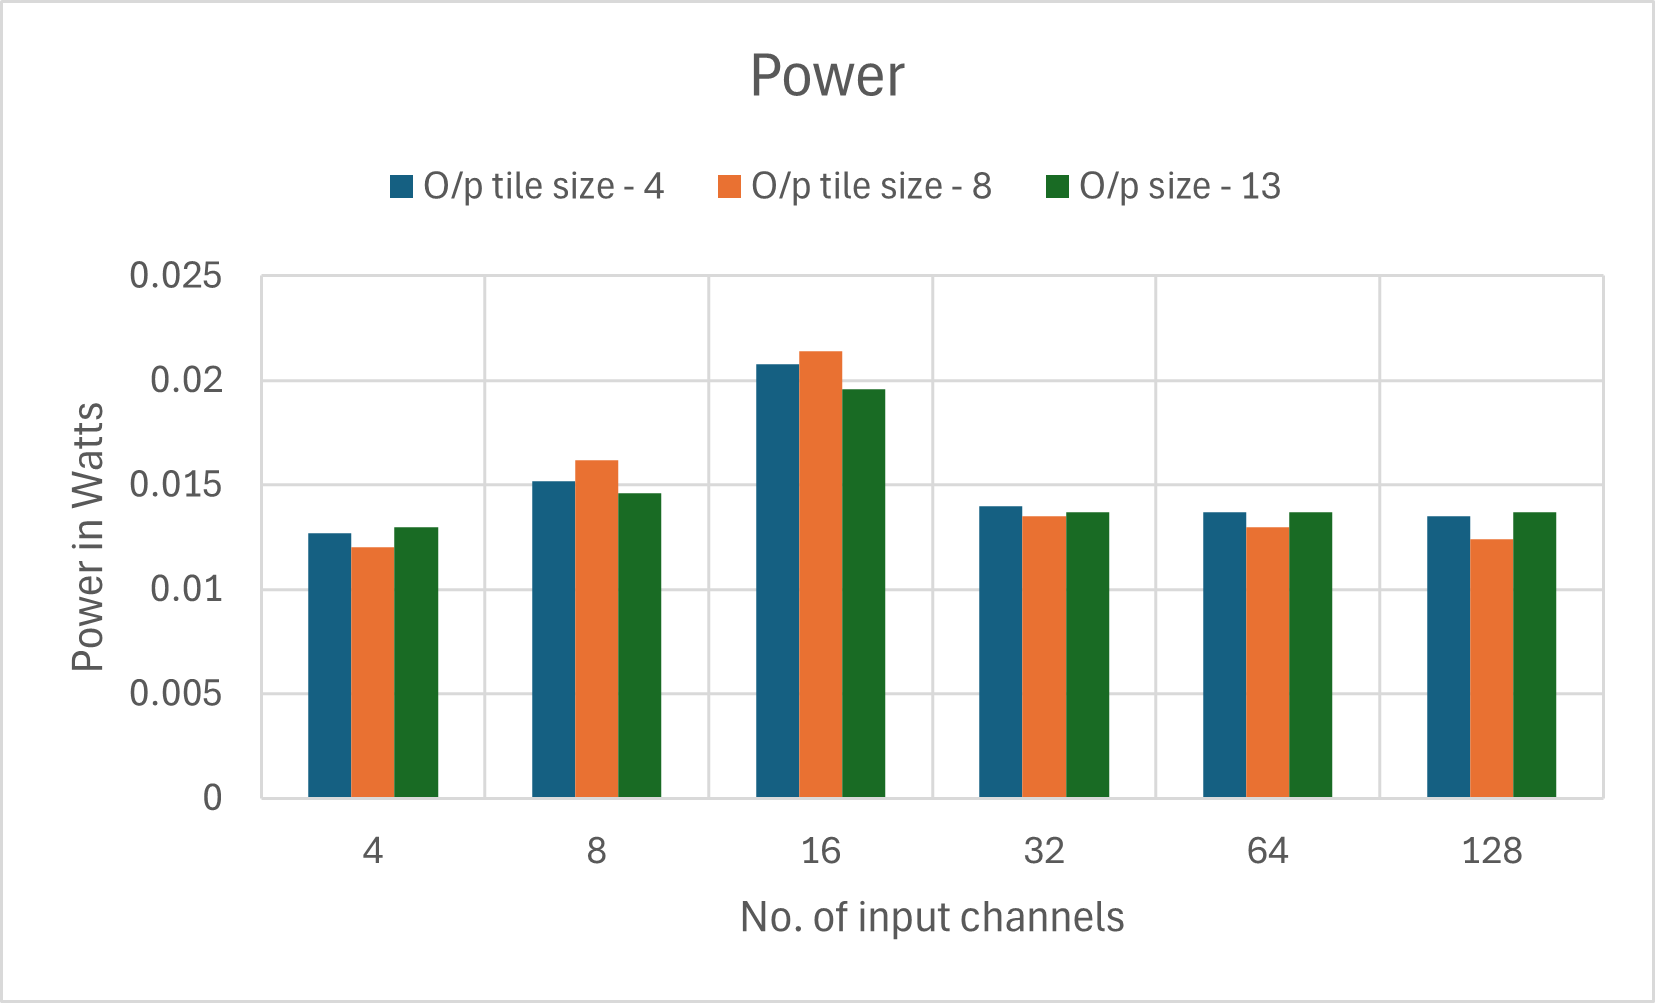
\includegraphics[width=\linewidth]{figure/chapter4_results/figure 1 - power.png}
   \caption{Power}
   \label{fig:power}
    \end{subfigure}
    \hfill
    \begin{subfigure}{0.45\textwidth}
   \centering
   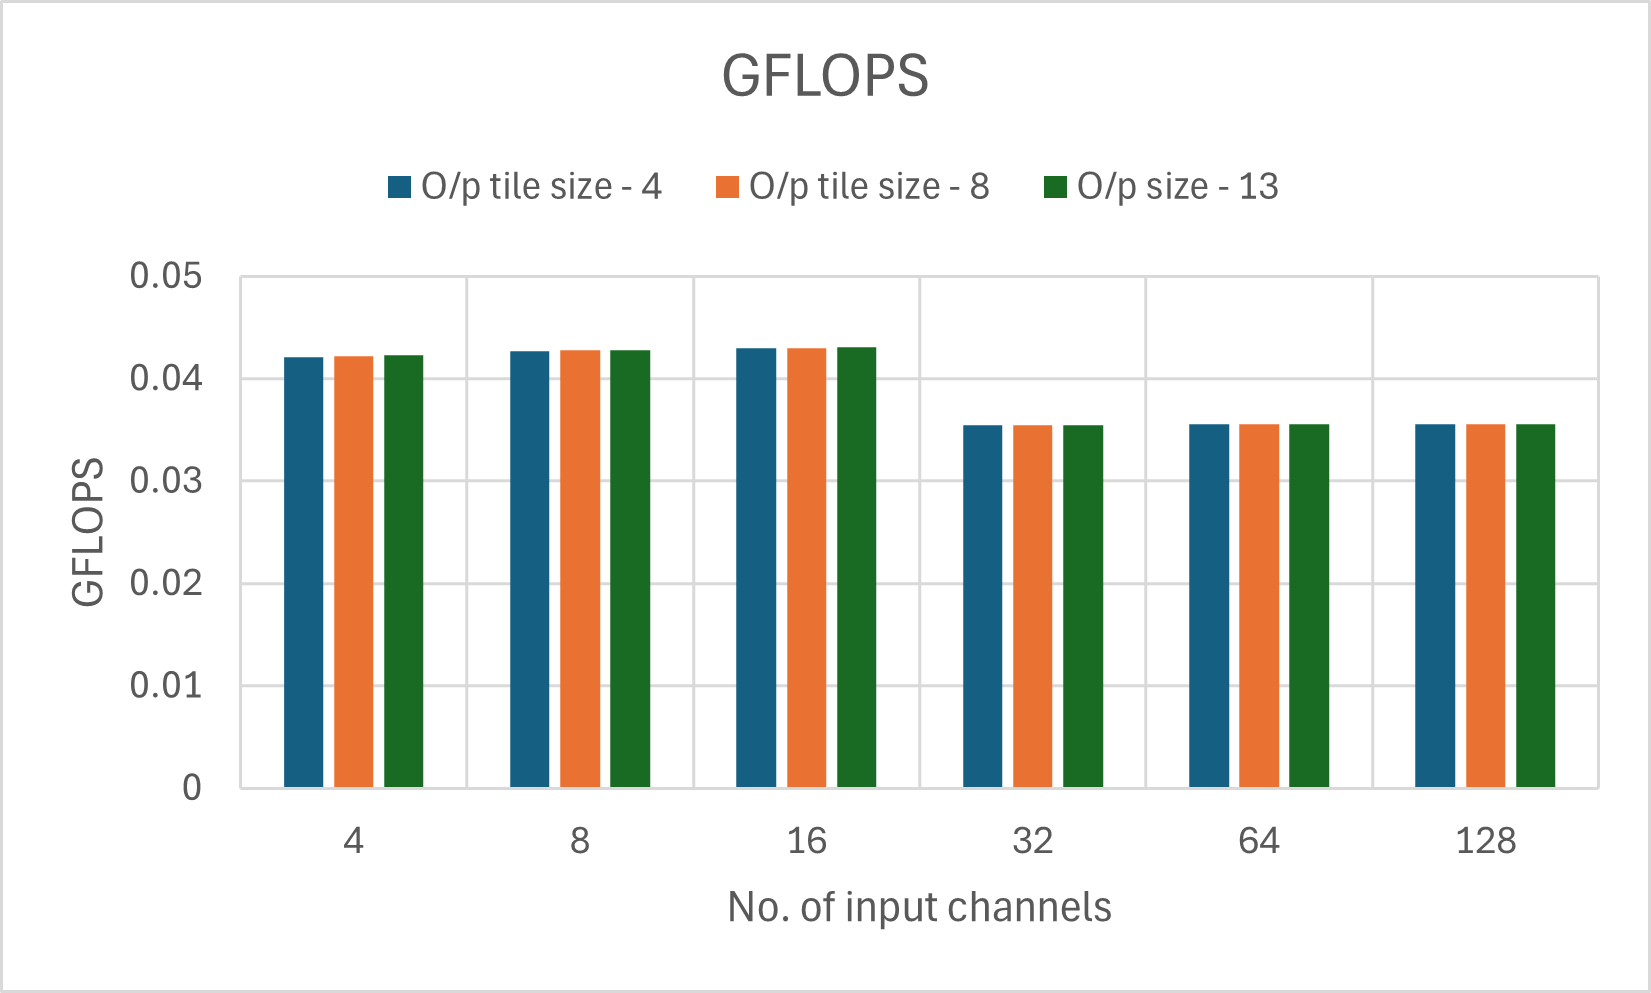
\includegraphics[width=\linewidth]{figure/chapter4_results/figure 2 - performance.png}
   \caption{Performance}
   \label{fig:performance}
    \end{subfigure}

    \vspace{0.5cm} % Space between rows

    % Second row: Area and Clock Cycles
    \begin{subfigure}{0.45\textwidth}
   \centering
   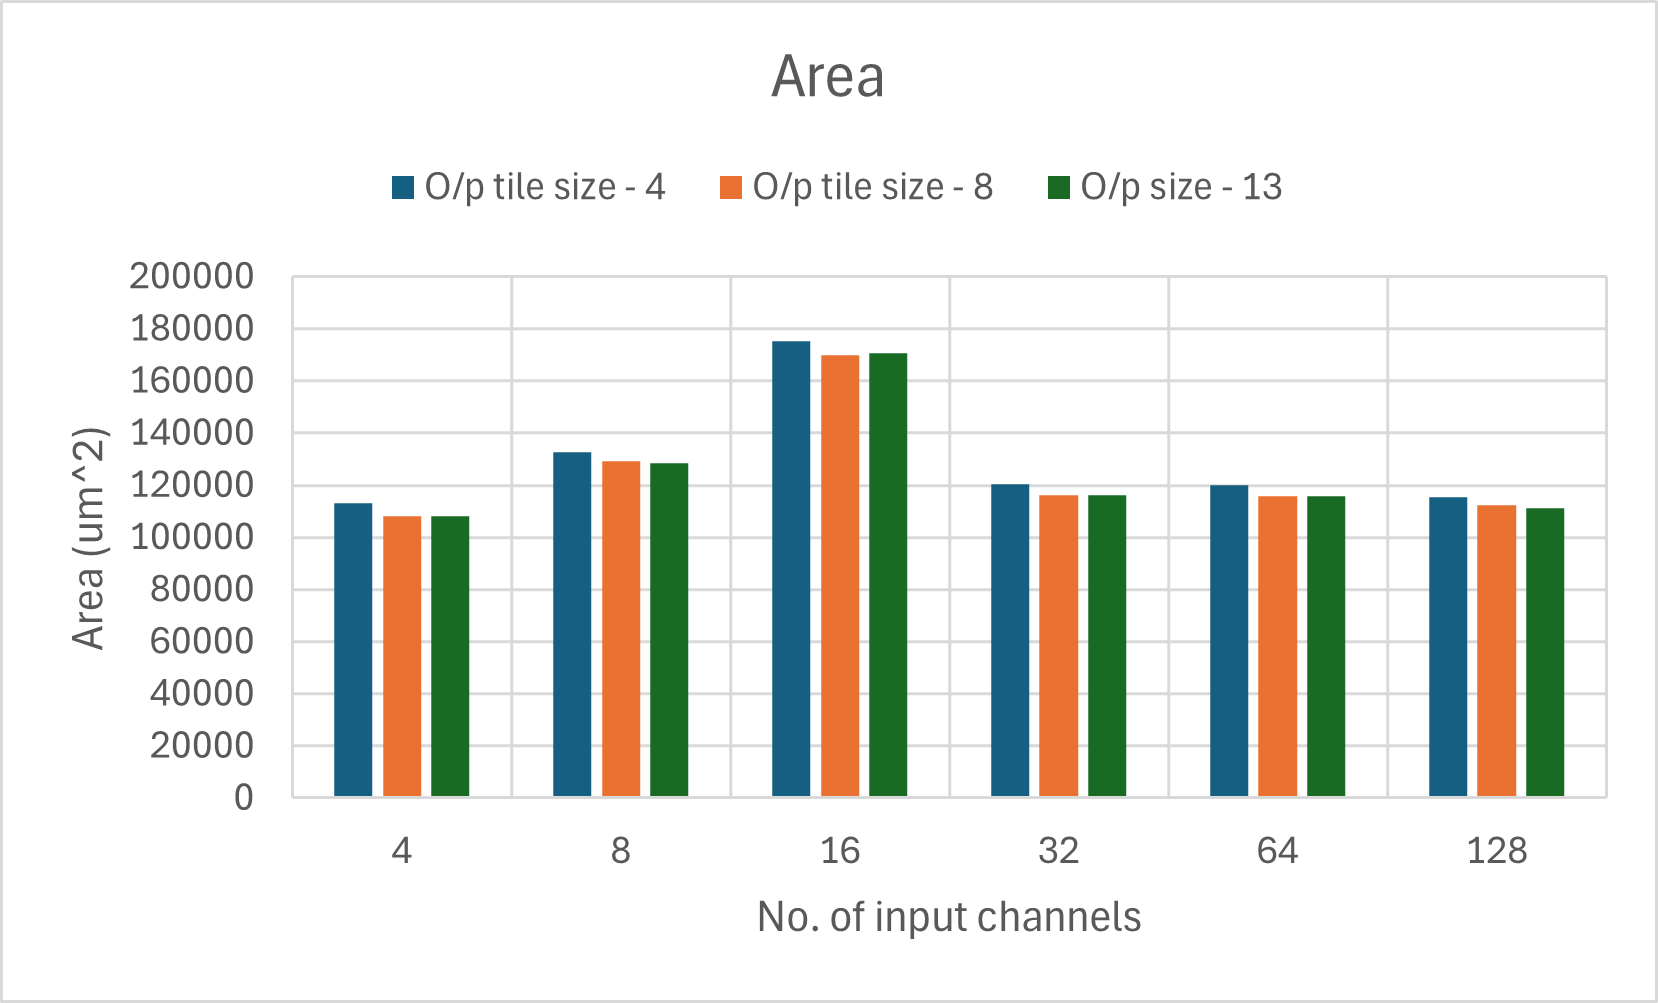
\includegraphics[width=\linewidth]{figure/chapter4_results/figure 3 - area.png}
   \caption{Area}
   \label{fig:area}
    \end{subfigure}
    \hfill
    \begin{subfigure}{0.45\textwidth}
   \centering
   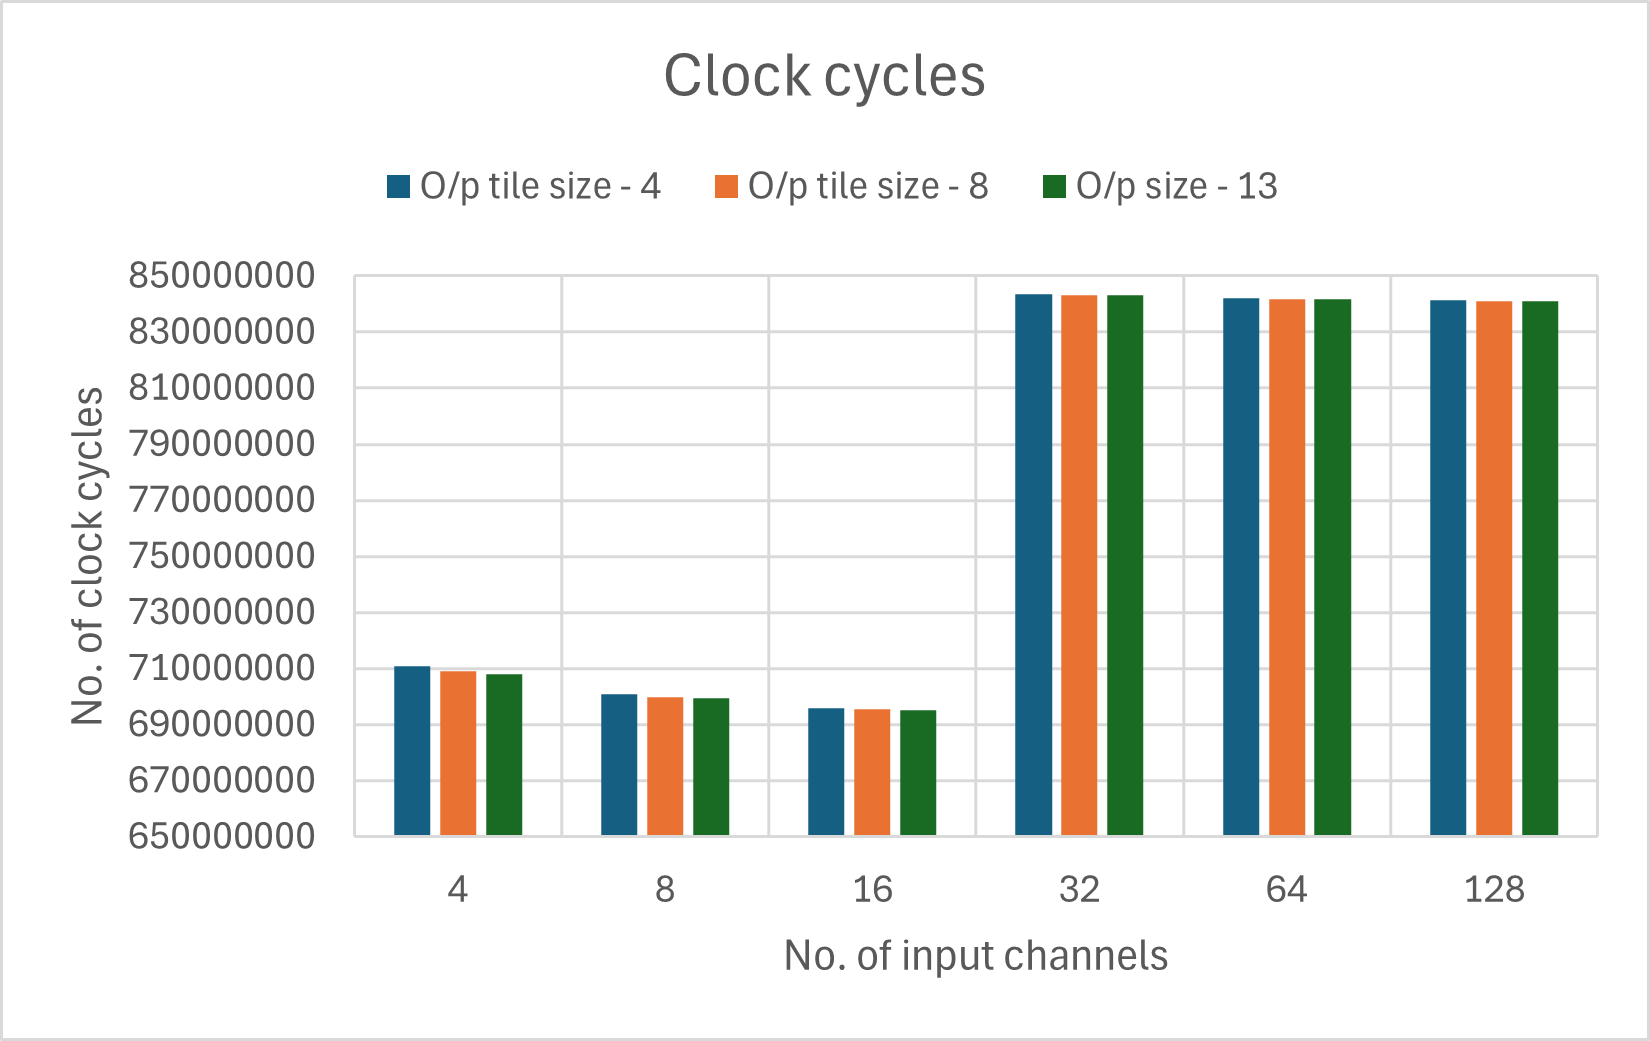
\includegraphics[width=\linewidth]{figure/chapter4_results/clockcycles.png}
   \caption{Clock Cycles}
   \label{fig:clock}
    \end{subfigure}

    \caption{Comparison of Power, Performance, Area, and Clock Cycles for different tiling configurations.}
    \label{fig:tileConvolutionCase2plot}
\end{figure}

The Figure \ref{fig:tileConvolutionCase2plot} illustrates the analysis of various tile configurations based on input channel sizes, focusing on key performance metrics such as power, performance (GFLOPS), area, and clock cycles. Such analysis is crucial for optimizing Convolution layer, as it helps identify the most efficient configurations to reduce the design space exploration. By examining these metrics, we can effectively narrow down the optimal tile sizes and input channel configurations, which are essential for improving computational performance while minimizing power, area, and resource usage.
\\
\begin{table}[H]
\centering
\caption{Loop tiling sweep}
\label{tab:tileConvolutionCase2Sweep}
\resizebox{\textwidth}{!}{%
 \begin{tabular}{|c|c|c|c|c|c|c|c|}
 \hline
 \textbf{Tile configuration} & 
 \textbf{Clock cycles}  & 
 \textbf{Total power} & 
 \textbf{Area} & 
 \textbf{Runtime} & 
 \textbf{GFLOPS} & 
 \textbf{GFLOPS/W} & 
 \textbf{Energy} \\ \hline
1,4,4,1,3,3,16 & 695,523,968 & 0.0208 & 175,114 & 6.9592 & 0.0429 & 2.0658 & 0.1447 \\ \hline
1,8,1,3,3,16   & 695,421,696 & 0.0214 & 169,841 & 6.9542 & 0.0430 & 2.0093 & 0.1488  \\ \hline
\rowcolor{yellow} 1,13,13,1,3,3,16 & 695,159,040 & 0.0196 & 170,582 & 6.9515 & 0.0430 & 2.1947 & 0.1362 \\ \hline
 \end{tabular}
}
\end{table}

 A sweep is performed across various tile configurations to identify the optimal combination of tile sizes for both the output and kernel. Table \ref{tab:tileConvolutionCase2Sweep} presents three different tile configurations, comparing their performance in terms of clock cycles, total power, area, runtime, GFLOPS, GFLOPS/W, and energy consumption. From this sweep, the configuration '1,13,13,1,3,3,16' was found to provide the best overall performance, with the lowest power and energy consumption, along with a balance in GFLOPS and GFLOPS/W.
\\

\begin{table}[H]
\centering
\caption{Loop tiling result}
\label{tab:tileConvolutionCase2Results}
\resizebox{\textwidth}{!}{%
 \begin{tabular}{|c|c|c|c|c|c|c|c|}
 \hline
 \textbf{Tile configuration} & 
 \textbf{Clock cycles}  & 
 \textbf{Total power} & 
 \textbf{Area} & 
 \textbf{Runtime} & 
 \textbf{GFLOPS} & 
 \textbf{GFLOPS/W} & 
 \textbf{Energy} \\ \hline
Baseline & 841,099,008 & 0.0137 & 111,099 & 8.4109 & 0.0355 & 2.5951 & 0.1152 \\ \hline
1,13,13,1,3,3,16 & 695,159,040 & 0.0196 & 170,582 & 6.9515 & 0.0430 & 2.1947 & 0.1362 \\ \hline
 \end{tabular}
}
\end{table}

In comparison to the baseline configuration (Table 2), the optimized tile configuration reduces clock cycles from 841,099,008 to 695,159,040 and improves runtime by nearly 1.5 seconds (from 8.41 to 6.95 seconds), at the cost of increased total power (from 0.0137 to 0.0196) and area (from 111,099 to 170,582). While GFLOPS improves from 0.0355 to 0.0430, GFLOPS/W decreases slightly, reflecting reduced power efficiency. The energy consumption also rises from 0.1152 to 0.1362, indicating the higher resource demand of the optimized configuration, which offers significant performance gains but at the expense of power and area.

\subsubsection{Case 3: Kernel height/width tiling.}

\begin{table}[H]
\centering
\caption{AlexNet Convolution layer-2 dimensions}
\label{tab:tileConvolutionCase3Dim}
 \begin{tabular}{|c|c|c|c|c|c|c|c|c|c|c|} \hline  
 
 \multirow{2}{*}{\textbf{Layer dimensions}} &  
 \multicolumn{3}{|c|}{\textbf{Input}} &  
 \multicolumn{4}{|c|}{\textbf{Kernel}} &  
 \multicolumn{3}{|c|}{\textbf{Output}}\\ \cline{2-11}
 & H &  W &  C&  H &  W &  C &  F &  H &  W & F\\ \hline  
 \textbf{Actual layer} &  31 & 31 & 96 & 5 & 5 & 96 & 256 & 27 & 27 & 256\\ \hline 
 \textbf{Executed layer} & 31 & 31 & \cellcolor{yellow}32 & 5 & 5 & \cellcolor{yellow}32 & \cellcolor{yellow}1 & 27 & 27 & \cellcolor{yellow}1 \\ \hline 
 \end{tabular}
\end{table}

The Table \ref{tab:tileConvolutionCase3Dim} shows the configuration details for AlexNet Convolution Layer 2 in both the actual and executed forms. The actual configuration has 96 input channels and 96 kernel channels, while the executed configuration reduces both the input and kernel channels to 32 for optimization. The output dimensions remain the same, with 27 x 27 spatial resolution for both configurations, but the number of output channels is reduced from 256 to 1 in the executed version. 
\\
\begin{table}[H]
\centering
\caption{Kernel tiled to size 3.}
\label{tab:tileConvolutionCase3KernelTile}
\resizebox{\textwidth}{!}{%
 \begin{tabular}{|c|c|c|c|c|c|c|c|}
 \hline
 \textbf{Tile configuration} & 
 \textbf{Clock cycles}  & 
 \textbf{Total power} & 
 \textbf{Area} & 
 \textbf{Runtime} & 
 \textbf{GFLOPS} & 
 \textbf{GFLOPS/W} & 
 \textbf{Energy} \\ \hline
 1,8,8,1,3,3,4 & 2,059,048,704 & 0.0156 & 142,327 & 20.5904 & 0.0435 & 2.7887 & 0.3212 \\ \hline
1,8,8,1,3,3,8 & 1,975,428,864 & 0.015 & 132,551 & 19.75429 & 0.045347 & 3.023133 & 0.2963 \\ \hline
1,8,8,1,3,3,16  & 1,933,594,368 & 0.0162 & 144,709 & 19.3359 & 0.0463 & 2.8597 & 0.3132 \\ \hline
1,8,8,1,3,3,32 & 2,360,451,840 & 0.0153 & 134,921 & 23.6045 & 0.0379 & 2.4803 & 0.3611 \\ \hline
 \end{tabular}
}
\end{table}

\begin{table}[H]
\centering
\caption{Kernel tiling is not applied.}
\label{tab:tileConvolutionCase3NoKernelTile}
\resizebox{\textwidth}{!}{%
 \begin{tabular}{|c|c|c|c|c|c|c|c|}
 \hline
 \textbf{Tile configuration} & 
 \textbf{Clock cycles}  & 
 \textbf{Total power} & 
 \textbf{Area} & 
 \textbf{Runtime} & 
 \textbf{GFLOPS} & 
 \textbf{GFLOPS/W} & 
 \textbf{Energy} \\ \hline
 1,8,8,1,5,5,4 & 1,911,125,760 & 0.0169 & 154,230 & 19.1112 & 0.0468 & 2.7735 & 0.3229 \\ \hline
1,8,8,1,5,5,8  & 1,912,603,392 & 0.0145 & 129,005 & 19.1260 & 0.0468 & 3.2300 & 0.2773 \\ \hline
1,8,8,1,5,5,16 & 1,902,144,768 & 0.0156 & 137,951 & 19.0214 & 0.0470 & 3.0188 & 0.2967 \\ \hline
1,8,8,1,5,5,32 & 2,347,600,128 & 0.0144 & 127,741 & 23.476 & 0.0381 & 2.6498 & 0.3380 \\ \hline
 \end{tabular}
}
\end{table}

Table \ref{tab:tileConvolutionCase3KernelTile} and Table \ref{tab:tileConvolutionCase3NoKernelTile} compare kernel tiling versus no kernel tiling for AlexNet Convolution Layer 2. For instance, the first configuration in Table \ref{tab:tileConvolutionCase3KernelTile} (1,8,8,1,3,3,4) shows 2,059,048,704 clock cycles, whereas the corresponding no-kernel-tiling configuration in Table \ref{tab:tileConvolutionCase3NoKernelTile} (1,8,8,1,5,5,4) reduces clock cycles to 1,911,125,760. Similarly, the second configuration with kernel tiling in Table \ref{tab:tileConvolutionCase3KernelTile} (1,8,8,1,3,3,8) has 1,975,428,864 clock cycles, while the no-kernel-tiling counterpart in Table \ref{tab:tileConvolutionCase3NoKernelTile} (1,8,8,1,5,5,8) lowers it to 1,912,603,392. This pattern of higher clock cycles with kernel tiling is consistent.

Overall, kernel tiling leads to degraded performance and should be avoided in such configurations.

\subsection{Depth-wise Convolution (Depth-wise Convolution) Layer}

\begin{table}[H]
\centering
\caption{Mobilenet-v3-small Depth-wise Convolution layer 2:}
\label{tab:tileDConvolutionDim}
 \begin{tabular}{|c|c|c|c|c|c|c|c|c|c|c|} \hline  
 
 \multirow{2}{*}{\textbf{Layer dimensions}} &  
 \multicolumn{3}{|c|}{\textbf{Input}} &  
 \multicolumn{3}{|c|}{\textbf{Kernel}} &  
 \multicolumn{3}{|c|}{\textbf{Output}}\\ \cline{2-10}
 & H &  W &  C&  H &  W &  C &  H &  W & F\\ \hline  
 \textbf{Actual layer} &  57 &  57 & 72 & 3 & 3 & 72 & 28 & 28 & 72\\ \hline 
 \textbf{Executed layer} &  57 &  57 &  \cellcolor{yellow}8 & 3 & 3 & \cellcolor{yellow}8 & 28 & 28 & \cellcolor{yellow}8 \\ \hline 
 \end{tabular}
\end{table}

Table \ref{tab:tileDConvolutionDim} provides the details for Mobilenet-v3-small Depth-wise Convolution Layer 2, displaying the dimensions of the input, kernel, and output for both the actual and executed configurations. In the actual configuration, the input and kernel channels are set to 72, while the executed configuration reduces the input and kernel channels to 8, optimizing the computation while maintaining the spatial dimensions of 57 x 57 for input and 28 x 28 for output.

\begin{table}[H]
\centering
\caption{Loop tiling result}
\label{tab:tileDConvolutionResults}
\resizebox{\textwidth}{!}{%
 \begin{tabular}{|c|c|c|c|c|c|c|c|}
 \hline
 \textbf{Tile configuration} & 
 \textbf{Clock cycles}  & 
 \textbf{Total power} & 
 \textbf{Area} & 
 \textbf{Runtime} & 
 \textbf{GFLOPS} & 
 \textbf{GFLOPS/W} & 
 \textbf{Energy} \\ \hline
Baseline & 2,949,318 & 0.013 & 107,069 & 0.029493 & 0.0344 & 2.6500 & 0.0003 \\ \hline
1,4,4,4,3,3 & 2,978,676 & 0.0133 & 110,727 & 0.0297 & 0.0341 & 2.5647 & 0.0003 \\ \hline
1,4,4,8,3,3 & 2,960,154 & 0.0131 & 110,486 & 0.0296 & 0.0343 & 2.6201 & 0.0003 \\ \hline
1,8,8,4,3,3 & 2,977,038 & 0.0143 & 112,763 & 0.0297 & 0.0341  & 2.3867 & 0.0004 \\ \hline
1,8,8,8,3,3 & 2,959,470 & 0.0135 & 111,279 & 0.0295 & 0.0343 & 2.5431 & 0.0004 \\ \hline
1,16,16,4,3,3 & 2,972,376 & 0.013 & 107,194 & 0.0297 & 0.0341 & 2.6294 & 0.0003 \\ \hline
 \end{tabular}
}
\end{table}

Table \ref{tab:tileDConvolutionResults} compares the clock cycles for different tiling configurations against the baseline. All tiling configurations show a slight increase in clock cycles compared to the baseline, which has 2,949,318 clock cycles. The highest observed value is 2,978,676 clock cycles, indicating that loop tiling does not improve performance and, in fact, results in a marginal degradation across all configurations.

The results demonstrate that loop tiling does not enhance performance for depthwise convolution layers, as every tile configuration tested increases the number of clock cycles compared to the baseline. Despite different tiling strategies, the performance degradation suggests that tiling may not be an effective optimization technique for this specific layer configuration.

\subsection{Fully Connected (FC) Layer}

\begin{table}[H]
\centering
\caption{AlexNet Fully Connected (FC) layer 3:}
\label{tab:tileFcDim}
 \begin{tabular}{|c|c|c|c|c|c|c|c|c|c|c|} \hline  
 
 \multirow{2}{*}{\textbf{Layer dimensions}} &  
 \multicolumn{2}{|c|}{\textbf{Input}} &  
 \multicolumn{2}{|c|}{\textbf{Weights}} &  
 \multicolumn{2}{|c|}{\textbf{Output}}\\ \cline{2-7}
 & H &  W &  H &  W & H &  W\\ \hline  
 \textbf{Actual layer} &  1 &  4096 & 4096 & 1000 & 1 & 1000 \\ \hline 
 \textbf{Executed layer} &  1 &  \cellcolor{yellow}128 & \cellcolor{yellow}128 & \cellcolor{yellow}125 & 1 & \cellcolor{yellow}125 \\ \hline 
 \end{tabular}
\end{table}

Table \ref{tab:tileFcDim} shows the dimensions for the input, weights, and output in both the actual and executed configurations. The actual configuration uses large dimensions of 4096 x 4096 for the weights and 1 x 1000 for the output. However, in the executed configuration, these dimensions are significantly reduced to 128 x 128 for the weights and 1 x 125 for the output.

\begin{table}[H]
\centering
\caption{Loop tiling - Sweep 1 (Inner-most loop)}
\label{tab:tileFcSweep1}
\resizebox{\textwidth}{!}{%
 \begin{tabular}{|c|c|c|c|c|c|c|c|}
 \hline
 \textbf{Tile configuration} & 
 \textbf{Clock cycles}  & 
 \textbf{Total power} & 
 \textbf{Area} & 
 \textbf{Runtime} & 
 \textbf{GFLOPS} & 
 \textbf{GFLOPS/W} & 
 \textbf{Energy} \\ \hline
1,1,4,4 & 35,244,032 & 0.0059 & 51,098 & 0.3524 & 0.0232 & 3.9396 & 0.0020  \\ \hline
1,1,4,8 & 33,314,816 & 0.0074 & 62,642 & 0.3331 & 0.0245 & 3.2874 & 0.0024  \\ \hline
\rowcolor{yellow} 1,1,4,16 & 32,350,208 & 0.0097 & 83,972 & 0.3235 & 0.0253 & 2.5892 & 0.0016 \\ \hline
1,1,4,32 & 39,007,488 & 0.0063 & 55,984 & 0.3900 & 0.0210 & 3.3142 & 0.0024 \\ \hline
1,1,4,64 & 34,655,488 & 0.0048 & 43,138 & 0.3465 & 0.0236 & 4.8838 & 0.0016 \\ \hline
1,1,4,128 & 34,527,488 & 0.0047 & 37,766 & 0.3452 & 0.0237 & 5.0373 & 0.0016 \\ \hline
 \end{tabular}
}
\end{table}

\begin{table}[H]
\centering
\caption{Loop tiling - Sweep 2 (Outer loop)}
\label{tab:tileFcSweep2}
\resizebox{\textwidth}{!}{%
 \begin{tabular}{|c|c|c|c|c|c|c|c|}
 \hline
 \textbf{Tile configuration} & 
 \textbf{Clock cycles}  & 
 \textbf{Total power} & 
 \textbf{Area} & 
 \textbf{Runtime} & 
 \textbf{GFLOPS} & 
 \textbf{GFLOPS/W} & 
 \textbf{Energy} \\ \hline
1,1,4,16 & 32,350,208 & 0.0097 & 83,972 & 0.3235 & 0.0253 & 2.5892 & 0.0031 \\ \hline
1,1,8,16 & 31,719,424 & 0.0097 & 84,101 & 0.3171 & 0.0258 & 2.6379 & 0.0031 \\ \hline
1,1,16,16 & 31,404,032 & 0.0099 & 84,888 & 0.314 & 0.0260 & 2.6296 & 0.0031 \\ \hline
1,1,32,16 & 31,246,336 & 0.0098 & 84,589 & 0.3124 & 0.0262 & 2.6671 & 0.0030 \\ \hline
\rowcolor{yellow} 1,1,64,16 & 31,124,736 & 0.0142 & 118,464 & 0.3112 & 0.0263 & 1.8535 & 0.0044 \\ \hline
1,1,125,16 & 31,125,504 & 0.0095 & 80,886 & 0.3112 & 0.0263 & 2.7530 & 0.0029 \\ \hline
 \end{tabular}
}
\end{table}

The methodology involves a two-step tiling process to optimize the performance of a fully connected (FC) layer. In the first sweep, different tile configurations for the innermost loop were tested, as shown in Table \ref{tab:tileFcSweep1}. The tile configuration '1,1,4,16' provided the best performance, minimizing clock cycles to 32,350,208. Following this, the second sweep focused on tiling the outer loop, with the innermost loop tile fixed at 16, as detailed in Table \ref{tab:tileFcSweep2}. Here, the tile configuration '1,1,64,16' resulted in further reduction of clock cycles to 31,124,736, though with a higher power consumption (0.0142 W) and energy usage (0.0044197074 J).
\\
\begin{table}[H]
\centering
\caption{Loop tiling result}
\label{tab:tileFcResult}
\resizebox{\textwidth}{!}{%
 \begin{tabular}{|c|c|c|c|c|c|c|c|}
 \hline
 \textbf{Tile configuration} & 
 \textbf{Clock cycles}  & 
 \textbf{Total power} & 
 \textbf{Area} & 
 \textbf{Runtime} & 
 \textbf{GFLOPS} & 
 \textbf{GFLOPS/W} & 
 \textbf{Energy} \\ \hline
Baseline & 34,511,104 & 0.0045 & 36,055 & 0.3451 & 0.0237 & 5.2284 & 0.0015 \\ \hline
1,1,64,16 & 31,124,736 & 0.0142 & 118,464 & 0.3112 & 0.0263 & 1.8535 & 0.0044 \\ \hline
 \end{tabular}
}
\end{table}

he comparison between the baseline configuration and the best configuration is shown in the Table \ref{tab:tileFcResult}. The baseline configuration has 34,511,104 clock cycles, a total power of 0.0045 W, and an area of 36,055 $\mu\text{m}^2$, with a runtime of 0.3451 seconds. In contrast, the best configuration, '1,1,64,16', reduces the clock cycles to 31,124,736 and the runtime to 0.3112 seconds, but increases total power to 0.0142 W and area to 118,464 $\mu\text{m}^2$. While the best configuration improves performance in terms of clock cycles and runtime, it comes at the cost of higher power consumption and area. Additionally, GFLOPS improves slightly, but GFLOPS/W and energy efficiency are reduced compared to the baseline.

\clearpage
\section{Loop Unrolling}
\subsection{Convolution (Convolution) Layer}

Loop unrolling for Convolution layer has 3 cases:
\begin{enumerate}
 \item Unrolling smaller kernel width/height with no. of input channels 1.
 \item Unrolling larger kernel width/height with no. of input channels 1.
 \item Unrolling kernels with no. of input channels $>$ 1.
\end{enumerate}

\subsubsection{Case 1 : Unrolling smaller kernel width/height with no. of input channels 1.}

\begin{table}[H]
\centering
\caption{LeNet-5 Convolution layer-1 dimensions}
\label{tab:unrollConvolutionCase1Dim}
 \begin{tabular}{|c|c|c|c|c|c|c|c|c|c|c|} \hline  
 
 \multirow{2}{*}{\textbf{Layer dimensions}} &  
 \multicolumn{3}{|c|}{\textbf{Input}} &  
 \multicolumn{4}{|c|}{\textbf{Kernel}} &  
 \multicolumn{3}{|c|}{\textbf{Output}}\\ \cline{2-11}
 & H &  W &  C&  H &  W &  C &  F &  H &  W & F\\ \hline  
 \textbf{Actual layer} &  32 &  32 &  1 & 5 & 5 & 1 & 6 & 28 & 28 & 6\\ \hline 
 \textbf{Executed layer} &  32 & 32 & 1 & 5 & 5 & 1 & \cellcolor{yellow}1 & 28 & 28 & \cellcolor{yellow}1 \\ \hline 
 \end{tabular}
\end{table}

In Table \ref{tab:unrollConvolutionCase1Dim}, the dimensions for the first convolutional layer (Convolution) of the LeNet-5 architecture are provided. The actual layer has an input size of 32 x 32 x 1, a kernel of 5 x 5 x 1, and an output of 28 x 28 x 6. In the executed layer, the number of output filters is set to 1.
\\
\begin{table}[H]
\centering
\caption{Loop unrolling results}
\label{tab:unrollConvolutionCase1Results}
\resizebox{\textwidth}{!}{%
 \begin{tabular}{|c|c|c|c|c|c|c|c|c|}
 \hline
 \textbf{No. of unrolls} &
 \textbf{Unroll-factor} &
 \textbf{Clock cycles}  & 
 \textbf{Total power} & 
 \textbf{Area} & 
 \textbf{Runtime} & 
 \textbf{GFLOPS} & 
 \textbf{GFLOPS/W} & 
 \textbf{Energy} \\ \hline
    0 & 0  & 362,712 & 0.0076 & 63,115 & 0.0036 & 0.0648 & 8.4989 & 2.7674e-05 \\ \hline
    1 & Full-unroll & 362,712 & 0.0076 & 62,464 & 0.0036 & 0.0648 & 8.4989 & 2.7674e-05 \\ \hline
    2 & 4  & 362,712 & 0.0073 & 62,752 & 0.0036 & 0.0648 & 8.8227 & 2.6658e-05 \\ \hline
    2 & Full-unroll & 362,712 & 0.0073 & 63,002 & 0.0036 & 0.0648 & 8.8709 & 2.6531e-05 \\ \hline
    3 & 4  & 362,712 & 0.0075 & 65,839 & 0.0036 & 0.0648 & 8.5550 & 2.7492e-05  \\ \hline
    3 & Full-unroll & 362,712 & 0.0077 & 65,821 & 0.0036 & 0.0648 & 8.3998  & 2.8000e-05  \\ \hline
 \end{tabular}
}
\end{table}

In Table \ref{tab:unrollConvolutionCase1Results}, the results of a loop unrolling experiment are presented, focusing on the case where the kernel width/height is small, and the number of input channels equals 1. Various configurations of no. of unrolls (0, 1, 2, and 3) were tested. The results show that performance does not improve with unrolling. Across all configurations, the clock cycles remain unchanged at 362,712, and there is no notable difference in runtime (0.0648 seconds) or GFLOPS (0.0648). While there are slight fluctuations in GFLOPS/W (ranging from 8.3998 to 8.8709) and total power, these differences are marginal and do not result in a significant improvement in performance. The energy consumption remains relatively stable, this confirms that loop unrolling offers no performance benefit for this specific layer configuration with a smaller kernel and a single input channel.


\subsubsection{Case 2 : Unrolling larger kernel width/height with no. of input channels 1.}

\begin{table}[H]
\centering
\caption{AlexNet Convolution layer-1 dimensions}
\label{tab:unrollConvolutionCase2Dim}
 \begin{tabular}{|c|c|c|c|c|c|c|c|c|c|c|} \hline  
 
 \multirow{2}{*}{\textbf{Layer dimensions}} &  
 \multicolumn{3}{|c|}{\textbf{Input}} &  
 \multicolumn{4}{|c|}{\textbf{Kernel}} &  
 \multicolumn{3}{|c|}{\textbf{Output}}\\ \cline{2-11}
 & H &  W &  C&  H &  W &  C &  F &  H &  W & F\\ \hline  
 \textbf{Actual layer} &  227 &  227 &  3 & 11 & 11 & 3 & 96 & 55 & 55 & 96\\ \hline 
 \textbf{Executed layer} &  227 &  227 &  \cellcolor{yellow}1 & 11 & 11 & \cellcolor{yellow}1 & \cellcolor{yellow}1 & 55 & 55 & \cellcolor{yellow}1 \\ \hline 
 \end{tabular}
\end{table}

In Table \ref{tab:unrollConvolutionCase2Dim}, the dimensions for the first convolutional layer (Convolution) in the AlexNet architecture are shown, focusing on the case of unrolling a larger kernel width/height with a number of input channels equal to 1. The actual layer has an input size of 227 x 227 x 3, a kernel size of 11 x 11 x 3, and produces an output of 55 x 55 x 96. However, in the executed layer, the number of input channels and kernel channels are reduced to 1, while the spatial dimensions of the input, kernel, and output remain the same.

\begin{table}[H]
\centering
\caption{Loop unrolling results}
\label{tab:unrollConvolutionCase2Results}
\resizebox{\textwidth}{!}{%
 \begin{tabular}{|c|c|c|c|c|c|c|c|c|}
 \hline
 \textbf{No. of unrolls} &
 \textbf{Unroll-factor} &
 \textbf{Clock cycles}  & 
 \textbf{Total power} & 
 \textbf{Area} & 
 \textbf{Runtime} & 
 \textbf{GFLOPS} & 
 \textbf{GFLOPS/W} & 
 \textbf{Energy} \\ \hline
0 & 0   & 425,162,016 & 0.0039 & 39,522 & 4.2516  & 0.0495 & 12.4592 & 0.0169  \\ \hline
1 & Full-unroll & 425,162,016 & 0.004   & 39,614 & 4.2516  & 0.0495 & 12.397    & 0.0170    \\ \hline
2 & 4   & 425,162,016 & 0.004   & 39,607 & 4.2516  & 0.0495 & 12.397    & 0.0170    \\ \hline
2 & 8   & 425,162,016 & 0.004   & 39,542 & 4.2516  & 0.0495 & 12.397    & 0.0170    \\ \hline
2 & Full-unroll & 425,162,016 & 0.0039 & 39,395 & 4.2516  & 0.0495 & 12.5539 & 0.0167  \\ \hline
3 & 4   & 396,422,208 & 0.0168  & 152,200 & 3.9642 & 0.0531 & 3.1656  & 0.0665  \\ \hline
3 & 8   & 318,195,072 & 0.0312  & 251,698 & 3.1819 & 0.0662 & 2.1236  & 0.0992  \\ \hline
3 & Full-unroll & 318,350,592 & 0.0322  & 248,566 & 3.1835 & 0.0662 & 2.0567  & 0.1025  \\ \hline
 \end{tabular}
}
\end{table}

Table \ref{tab:unrollConvolutionCase2Results} presents the results of the loop unrolling experiment for the first convolutional layer in AlexNet, which has a larger kernel size. The analysis was performed for different numbers of unrolls, including 0, 1, 2, and 3, with a mix of partial and full unroll configurations.
\begin{itemize}
    \item No. of unrolls = 0: This baseline case shows 425,162,016 clock cycles, with a runtime of 4.2516 seconds. The total power consumption is 0.0039 W, and the GFLOPS is 0.0495, resulting in GFLOPS/W of 12.4592. The energy consumption is 0.0169 J, and the area used is 39,522 $\mu\text{m}^2$. These values set the baseline for comparison with the unrolled cases.
    \item No. of unrolls = 1 (Full-unroll): The results with full unrolling for 1 iteration show no improvement over the baseline. The clock cycles, runtime, GFLOPS, and GFLOPS/W remain the same as the baseline, indicating that full unrolling for one iteration has no performance benefit. Total power and energy consumption are almost identical to the baseline, and only a slight reduction in area is observed (down to 39,614 $\mu\text{m}^2$).
    \item No. of unrolls = 2: With 2 unrolls, the clock cycles remain unchanged at 425,162,016, and other metrics like GFLOPS, runtime, and energy consumption show no notable improvements. Even with full unrolling, the results are nearly identical to the baseline. The area remains consistent at around 39,522 $\mu\text{m}^2$, further confirming that unrolling for two iterations offers no performance gain.
    \item No. of unrolls = 3: When moving to 3 unrolls, a significant difference is observed. The clock cycles decrease to 318,350,592, and the runtime improves to 3.1835 seconds, showing a substantial performance enhancement. This case also results in a higher GFLOPS of 0.0662 and a lower energy consumption of 0.0125, indicating better efficiency. However, the total power slightly increases to 0.0032, and the GFLOPS/W drops to 2.0567 from the baseline. The area usage also increases significantly to 248,656 $\mu\text{m}^2$, reflecting the trade-off in area usage for improved performance.
\end{itemize}

The results of the loop unrolling experiment highlight that unrolling larger kernels with a single input channel offers performance gains only when the unroll factor increases to 3. In earlier cases (0, 1, and 2 unrolls), there is no improvement in clock cycles, runtime, or other performance metrics. Even full unrolling does not yield any gains until the unroll count reaches 3. At this point, the significant reduction in clock cycles and improved runtime showcase the advantage of unrolling for large kernels, though at the cost of increased area and a slight reduction in GFLOPS/W. This suggests that unrolling is only beneficial for larger unroll factors and comes with trade-offs, particularly in area usage.

\subsubsection{Case 3 : Unrolling kernels with no. of input channels $>$ 1.}

\begin{table}[H]
\centering
\caption{AlexNet Convolution layer-5 dimensions}
\label{tab:unrollConvolutionCase3Dim}
 \begin{tabular}{|c|c|c|c|c|c|c|c|c|c|c|} \hline  
 
 \multirow{2}{*}{\textbf{Layer dimensions}} &  
 \multicolumn{3}{|c|}{\textbf{Input}} &  
 \multicolumn{4}{|c|}{\textbf{Kernel}} &  
 \multicolumn{3}{|c|}{\textbf{Output}}\\ \cline{2-11}
 & H &  W &  C&  H &  W &  C &  F &  H &  W & F\\ \hline  
 \textbf{Actual layer} &  15 &  15 & 384 & 3 & 3 & 384 & 256 & 13 & 13 & 256\\ \hline 
 \textbf{Executed layer} &  15 &  15 &  \cellcolor{yellow}32 & 3 & 3 & \cellcolor{yellow}32 & \cellcolor{yellow}1 & 13 & 13 & \cellcolor{yellow}1 \\ \hline 
 \end{tabular}
\end{table}

In Table \ref{tab:unrollConvolutionCase3Dim}, the dimensions for the fifth convolutional layer (Convolution) in AlexNet are shown under the case of unrolling kernels with more than one input channel. The actual layer has an input size of 15 x 15 x 384, a kernel size of 3 x 3 x 384, and an output of 13 x 13 x 256. However, during execution, the number of input and kernel channels are reduced to 32 and 1, respectively, and the output filters are also reduced to 1.
\\
\begin{table}[H]
\centering
\caption{Loop unrolling results}
\label{tab:unrollConvolutionCase3Results}
\resizebox{\textwidth}{!}{%
 \begin{tabular}{|c|c|c|c|c|c|c|c|c|}
 \hline
 \textbf{No. of unrolls} &
 \textbf{Unroll-factor} &
 \textbf{Clock cycles}  & 
 \textbf{Total power} & 
 \textbf{Area} & 
 \textbf{Runtime} & 
 \textbf{GFLOPS} & 
 \textbf{GFLOPS/W} & 
 \textbf{Energy} \\ \hline
0 & 0   & 750,243,840  & 0.0049 & 45,452  & 7.5024  & 0.0398 & 8.0199   & 0.0372 \\ \hline
1 & 4   & 603,319,296  & 0.0043 & 39,082  & 6.0331  & 0.0495 & 11.3683 & 0.0263 \\ \hline
1 & 8   & 606,434,304  & 0.0032 & 29,279  & 6.0643  & 0.0493 & 15.0798 & 0.0198 \\ \hline
1 & 16  & 606,434,304  & 0.0049 & 39,412  & 6.0643  & 0.0493 & 10.0429 & 0.0297 \\ \hline
1 & Full-unroll & 601,761,792  & 0.0075 & 65,218  & 6.0176  & 0.0496 & 6.5819  & 0.0454  \\ \hline
2 & Full-unroll & 600,204,288  & 0.0232  & 177,517 & 6.0020  & 0.0498 & 2.1475  & 0.1392  \\ \hline
3 & Full-unroll & 457,986,048  & 0.0649  & 509,320 & 4.5798   & 0.0652 & 1.0060  & 0.2972   \\ \hline

 \end{tabular}
}
\end{table}

Table \ref{tab:unrollConvolutionCase3Results} presents the results of the loop unrolling experiment for AlexNet Convolution Layer-5, where different numbers of unrolls (0, 1, 2, and 3) are tested, along with full unroll configurations for each.

\begin{itemize}
    \item No. of unrolls = 0 (Baseline): Without unrolling, the baseline configuration results in 750,243,840 clock cycles, with a total power consumption of 0.0049 W and an area usage of 45,452 $\mu\text{m}^2$. The runtime is 7.5024 seconds, and it achieves 0.0398 GFLOPS with a GFLOPS/W of 8.0199. The energy consumption stands at 0.0372 J. This serves as the baseline performance for comparison with the unrolled configurations.
    \item No. of unrolls = 1: When unrolling with a factor of 4, the clock cycles reduce significantly to 603,319,296, improving the runtime to 6.0331 seconds, with GFLOPS increasing to 0.0495 and GFLOPS/W to 11.3683. Additionally, total power decreases to 0.0043 W, and energy consumption drops to 0.0263 J. The area also decreases slightly to 39,082 $\mu\text{m}^2$, making this configuration both performance-efficient and area-efficient. For 8 unrolls, the clock cycles slightly increase to 606,434,304, with a runtime of 6.0643 seconds. While GFLOPS remains at 0.0493, GFLOPS/W is highest at 15.0798, and total power improves to 0.0032 W, but area remains stable at 29,279 $\mu\text{m}^2$. With 16 unrolls, performance remains similar to the 8-unroll case, showing diminishing returns with no further improvement in clock cycles, runtime, or area. In the full-unroll configuration, the clock cycles decrease slightly to 601,761,792, and runtime improves to 6.0167 seconds. However, GFLOPS/W drops to 6.5819, and both total power and energy consumption increase. The area expands to 65,218 $\mu\text{m}^2$, indicating that full unrolling at this level provides limited performance benefits but at a significantly higher area and energy cost.
    \item No. of unrolls = 2 (Unroll-factor = Full-unroll): With 2 full unrolls, the clock cycles further reduce to 600,204,288, and the runtime improves to 6.0202 seconds. GFLOPS stays consistent, but GFLOPS/W diminishes to 2.1475. Total power and area increase to 0.0322 W and 177,517 $\mu\text{m}^2$, respectively. Energy consumption increases to 0.1392 J, showing that this configuration provides a marginal performance improvement, but at the cost of significant increase in power and area.
    \item No. of unrolls = 3 (Unroll-factor = Full-unroll): At the highest level of unrolling with 3 full unrolls, the clock cycles reduce to 457,986,048, providing the best performance with the lowest runtime of 4.5798 seconds. The GFLOPS increases to 0.0652, but the GFLOPS/W drops to 1.0060, indicating that energy efficiency is compromised. Total power increases significantly to 0.0649 W, and energy consumption rises to 0.2972 J, showing that while unrolling improves performance, it comes at a higher energy and area cost.
\end{itemize}

As the number of unrolls increases, the clock cycles and runtime improve significantly, especially for 3 unrolls with full unrolling. However, these performance gains come at the expense of total power, area, and energy consumption. Unrolling once with a factor of 4 provides a good balance between performance improvements and efficiency, while further unrolling (8, 16, and full unroll) provides diminishing returns in terms of clock cycles and GFLOPS but leads to higher energy consumption and area usage. Therefore, optimal unrolling depends on the specific performance and power-efficiency goals for the application.


\subsection{Depth-wise Convolution (Depth-wise Convolution) Layer}


Loop permutation for Depth-wise Convolution layer has 2 cases:
\begin{enumerate}
 \item Kernels with no. of input channels 1.
 \item Kernels with no. of input channels $>$ 1.
\end{enumerate}


\subsubsection{Case 1: Kernels with number of input channels 1.}


\begin{table}[H]
\centering
\caption{Mobilenet-v3-small Depth-wise Convolution Layer 1:}
\label{tab:unrollDConvolutionCase1Dim}
 \begin{tabular}{|c|c|c|c|c|c|c|c|c|c|c|} \hline  
 
 \multirow{2}{*}{\textbf{Layer dimensions}} &  
 \multicolumn{3}{|c|}{\textbf{Input}} &  
 \multicolumn{3}{|c|}{\textbf{Kernel}} &  
 \multicolumn{3}{|c|}{\textbf{Output}}\\ \cline{2-10}
 & H &  W &  C&  H &  W &  C &  H &  W & F\\ \hline  
 \textbf{Actual layer} &  113 &  113 & 16 & 3 & 3 & 16 & 56 & 56 & 16\\ \hline 
 \textbf{Executed layer} &  113 &  113 &  \cellcolor{yellow}1 & 3 & 3 & \cellcolor{yellow}1 & 56 & 56 & \cellcolor{yellow}1 \\ \hline 
 \end{tabular}
\end{table}

Table \ref{tab:unrollDConvolutionCase1Dim} displays the dimensions of the first depthwise convolutional layer (Depth-wise Convolution) in the Mobilenet-v3-small architecture, under the case of kernels with a single input channel. The actual layer has an input size of 113 x 113 x 16, a kernel size of 3 x 3 x 16, and produces an output of 56 x 56 x 16. However, during execution, the number of input channels and output filters is reduced to 1.


\begin{table}[H]
\centering
\caption{Loop unrolling results}
\label{tab:unrollDNNCase1Results}
\resizebox{\textwidth}{!}{%
 \begin{tabular}{|c|c|c|c|c|c|c|c|c|}
 \hline
 \textbf{No. of unrolls} &
 \textbf{Unroll-factor} &
 \textbf{Clock cycles}  & 
 \textbf{Total power} & 
 \textbf{Area} & 
 \textbf{Runtime} & 
 \textbf{GFLOPS} & 
 \textbf{GFLOPS/W} & 
 \textbf{Energy} \\ \hline
0 & 0   & 1,456,192  & 0.0037 & 34,754  & 0.0145  & 0.0620 & 16.6725  & 5.42E-05  \\ \hline
1 & Full-unroll & 1,456,192  & 0.0039 & 35,817  & 0.0145  & 0.0620 & 15.8219  & 5.71E-05  \\ \hline
2 & Full-unroll & 1,457,088  & 0.0038  & 34,968  & 0.0145  & 0.0619 & 16.3115  & 5.54E-05  \\ \hline
3 & Full-unroll & 1,457,088  & 0.0038 & 34,985  & 0.0145  & 0.0619 & 16.2687  & 5.55E-05  \\ \hline
 \end{tabular}
}
\end{table}

Table \ref{tab:unrollDNNCase1Results} summarizes the results of loop unrolling for this layer. It is observed that performance worsens with more unrolling. As the number of unrolls increases, there are no significant improvements in clock cycles, runtime, or GFLOPS. In fact, the energy consumption and total power increase slightly, while the efficiency (GFLOPS/W) also decreases marginally. Therefore, higher unroll factors lead to worse performance and increased power and energy usage for this layer configuration.

\subsubsection{Case 2: Kernels with no. of input channels $>$ 1.}

\begin{table}[H]
\centering
\caption{Mobilenet-v3-small Depth-wise Convolution layer 2:}
\label{tab:unrollDConvolutionCase2Dim}
 \begin{tabular}{|c|c|c|c|c|c|c|c|c|c|c|} \hline  
 
 \multirow{2}{*}{\textbf{Layer dimensions}} &  
 \multicolumn{3}{|c|}{\textbf{Input}} &  
 \multicolumn{3}{|c|}{\textbf{Kernel}} &  
 \multicolumn{3}{|c|}{\textbf{Output}}\\ \cline{2-10}
 & H &  W &  C&  H &  W &  C &  H &  W & F\\ \hline  
 \textbf{Actual layer} &  57 &  57 & 72 & 3 & 3 & 72 & 28 & 28 & 72\\ \hline 
 \textbf{Executed layer} &  57 &  57 &  \cellcolor{yellow}24 & 3 & 3 & \cellcolor{yellow}24 & 28 & 28 & \cellcolor{yellow}24 \\ \hline 
 \end{tabular}
\end{table}

The table  \ref{tab:unrollDConvolutionCase2Dim} represents the performance of Mobilenet-v3-small D-Convolution Layer 2. The actual layer dimensions consist of an input size of 57 x 57 x 72, a kernel size of 3 x 3 x 72, and an output of 28 x 28 x 72. In the executed layer, the input and kernel channels are reduced to 24, which simplifies the computation.

\begin{table}[H]
\centering
\caption{Loop unrolling results}
\label{tab:unrollDConvolutionCase2Results}
\resizebox{\textwidth}{!}{%
 \begin{tabular}{|c|c|c|c|c|c|c|c|c|}
 \hline
 \textbf{No. of unrolls} &
 \textbf{Unroll-factor} &
 \textbf{Clock cycles}  & 
 \textbf{Total power} & 
 \textbf{Area} & 
 \textbf{Runtime} & 
 \textbf{GFLOPS} & 
 \textbf{GFLOPS/W} & 
 \textbf{Energy} \\ \hline
 0 & 0   & 2,203,914  & 0.0037 & 36,695  & 0.0220  & 0.0461 & 12.2289  & 8.31E-05  \\ \hline
1 & Full-unroll & 2,203,914  & 0.0037 & 36,261  & 0.0220  & 0.0461 & 12.2941  & 8.26E-05  \\ \hline
2 & Full-unroll & 2,203,914  & 0.0037 & 35,808  & 0.0220  & 0.0461 & 12.3270  & 8.24E-05  \\ \hline
3 & 4   & 1,357,194  & 0.0094 & 88,117  & 0.0135  & 0.0748 & 7.95589  & 0.000128  \\ \hline
3 & 8   & 1,230,186  & 0.0166  & 152,923 & 0.0123  & 0.0825 & 4.9754  & 0.000204  \\ \hline
3 & 16  & 1,173,036  & 0.042   & 343,284 & 0.0117   & 0.0866 & 2.0624  & 0.000493  \\ \hline
3 & Full-unroll & 645,180    & 0.0579  & 466,803 & 0.0064  & 0.1574  & 2.7198  & 0.000374  \\ \hline

 \end{tabular}
}
\end{table}

Table \ref{tab:unrollDConvolutionCase2Results} presents the performance metrics for different unrolling factors.
\begin{itemize}
    \item No. of unrolls = 0 (Baseline): The baseline configuration without unrolling shows 2,203,914 clock cycles with a runtime of 0.022039 seconds, achieving 0.046103 GFLOPS and a GFLOPS/W of 12.22891. The total power is 0.00377 W, and the area usage is 36,695 $\mu\text{m}^2$. This serves as the baseline for comparison.
    \item No. of unrolls = 1 (Full-unroll): This configuration provides no improvement in clock cycles or runtime, both of which remain the same as the baseline. There is a slight reduction in total power to 0.00375 and a minor improvement in GFLOPS/W, but the changes are negligible. This indicates that unrolling with 1 factor doesn't provide significant performance benefits.
    \item No. of unrolls = 2 (Full-unroll): Similar to the 1 unroll case, full unrolling for 2 unrolls offers little improvement in terms of performance, with clock cycles and runtime unchanged from the baseline.
    \item No. of unrolls = 3 (Unroll-factor = 4): Unrolling with a factor of 4 results in significant improvements. Clock cycles drop to 1,357,194, and runtime reduces to 0.013572 seconds, while GFLOPS increases to 0.074865. However, GFLOPS/W decreases to 7.955898, and the total power increases to 0.0094 W, with a notable rise in area to 88,117 $\mu\text{m}^2$. This configuration offers improved speed but at a higher cost in terms of power and area usage.
    \item No. of unrolls = 3 (Unroll-factor = 8): With a higher unroll factor of 8, the clock cycles reduce further to 1,230,186, and the runtime improves to 0.012302 seconds. GFLOPS rises to 0.0825, but GFLOPS/W drops to 4.9754, indicating reduced power efficiency. Total power increases to 0.0166 W, and area expands to 152,923 $\mu\text{m}^2$.
    \item No. of unrolls = 3 (Unroll-factor = 16): At an unroll factor of 16, the performance continues to improve in terms of speed. Clock cycles drop to 1,173,036, and runtime reduces to 0.01173 seconds. However, while GFLOPS reaches 0.086621, GFLOPS/W drops drastically to 2.062405. Total power spikes to 0.042 W, and area expands significantly to 343,284 $\mu\text{m}^2$.
    \item No. of unrolls = 3 (Full-unroll): Full unrolling with 3 unrolls provides the best speed performance, with clock cycles dropping to 645,180, and runtime improving to 0.006452 seconds. GFLOPS increases significantly to 0.15748, but GFLOPS/W drops sharply to 2.719862, indicating poor power efficiency. The total power rises to 0.0579 W, and area usage reaches 466,803 $\mu\text{m}^2$, the highest among all configurations.
    
\end{itemize}

The analysis shows that unrolling with a factor of 4 provides comparable results to full unrolling with 1 unroll in terms of total power, area, and GFLOPS/W, while offering better results in terms of clock cycles and speed. As unrolling factors increase beyond 4, clock cycles continue to decrease, improving speed, but at the expense of significantly higher total power, area, and energy consumption. The 3 full-unroll configuration delivers the best speed but at a substantial cost in power and area efficiency, making it less ideal for energy-constrained environments

\subsection{Fully Connected (FC) Layer}

\begin{table}[H]
\centering
\caption{AlexNet Fully Connected (FC) layer 1:}
\label{tab:unrollFcDim}
 \begin{tabular}{|c|c|c|c|c|c|c|c|c|c|c|} \hline  
 
 \multirow{2}{*}{\textbf{Layer dimensions}} &  
 \multicolumn{2}{|c|}{\textbf{Input}} &  
 \multicolumn{2}{|c|}{\textbf{Weights}} &  
 \multicolumn{2}{|c|}{\textbf{Output}}\\ \cline{2-7}
 & H &  W &  H &  W & H &  W\\ \hline  
 \textbf{Actual layer} &  1 &  9216 & 9216 & 4096 & 1 & 4096 \\ \hline 
 \textbf{Executed layer} &  1 &  \cellcolor{yellow}32 & \cellcolor{yellow}32 & \cellcolor{yellow}32 & 1 & \cellcolor{yellow}32 \\ \hline 
 \end{tabular}
\end{table}

The table \ref{tab:unrollFcDim}  AlexNet Fully Connected (FC) Layer dimensions. The actual layer has an input size of 1 x 9216, weights of 9216 x 4096, and an output of 1 x 4096. For the executed layer, the dimensions are reduced to 1 x 32 for the input, and output.

\begin{table}[H]
\centering
\caption{Loop unrolling results}
\label{tab:unrollFcResults}
\resizebox{\textwidth}{!}{%
 \begin{tabular}{|c|c|c|c|c|c|c|c|c|}
 \hline
 \textbf{No. of unrolls} &
 \textbf{Unroll-factor} &
 \textbf{Clock cycles}  & 
 \textbf{Total power} & 
 \textbf{Area} & 
 \textbf{Runtime} & 
 \textbf{GFLOPS} & 
 \textbf{GFLOPS/W} & 
 \textbf{Energy} \\ \hline
0 & 0   & 155,787,264  & 0.001  & 12,258   & 1.5578  & 0.0484 & 34.6157  & 0.0021 \\ \hline
1 & 4   & 118,038,528  & 0.008  & 70,710   & 1.1803  & 0.0639 & 7.2189   & 0.0104 \\ \hline
1 & 8   & 118,038,528  & 0.008  & 70,417   & 1.1803  & 0.0639 & 7.2027   & 0.0104 \\ \hline
1 & 16  & 118,038,528  & 0.008  & 71,035   & 1.1803  & 0.0639 & 7.1946   & 0.0104 \\ \hline
1 & Full-unroll & 118,038,528  & 0.008  & 70,921   & 1.1803  & 0.0639 & 7.2571   & 0.01041  \\ \hline
2 & 4   & 59,645,952   & 0.0228  & 178,788  & 0.5964  & 0.1265 & 5.5515   & 0.0135   \\ \hline
2 & 8   & 50,208,768   & 0.0383  & 323,216  & 0.5020  & 0.1503 & 3.9260   & 0.0192  \\ \hline
2 & 16  & 45,490,176   & 0.0711  & 575,059  & 0.4549  & 0.1659 & 2.3342   & 0.0323  \\ \hline
2 & Full-unroll & 43,057,152   & 0.166   & 1,146,979 & 0.4305 & 0.1753 & 1.0562   & 0.0714  \\ \hline
 \end{tabular}
}
\end{table}

The table \ref{tab:unrollFcResults} shows the performance results for the AlexNet Fully Connected (FC) Layer 1 when different unroll factors are applied. 

\begin{itemize}
    \item No. of Unrolls = 0 (Baseline): Without unrolling, the baseline configuration shows 155,787,264 clock cycles, with a total power consumption of 0.0014 W and an area of 12,258 $\mu\text{m}^2$. The runtime is 1.5578 seconds, and the GFLOPS achieved is 0.0484 with a GFLOPS/W of 34.6157. This baseline serves as the reference point for the performance of different unrolling configurations.
    \item No. of Unrolls = 1 (Unroll factors 4, 8, 16, and Full-unroll): For all configurations of 1 unroll, regardless of the unroll factor (4, 8, 16, or full), the performance remains unchanged. The clock cycles, runtime, and GFLOPS remain consistent across all cases, at 118,038,528 clock cycles, 1.1803 seconds runtime, and 0.0633 GFLOPS. The total power increases to 0.0088 W for all these configurations, and GFLOPS/W drops significantly to around 7.2 in each case. The area usage increases to around 70,000 $\mu\text{m}^2$ across all unroll factors. This indicates that unrolling with 1 factor, regardless of configuration, does not improve performance and results in increased power consumption without a corresponding speedup.
    \item No. of Unrolls = 2 (Unroll factor 4): Reduces the clock cycles to 59,645,952 and the runtime to 0.5964 seconds, while GFLOPS increases to 0.1265. However, the total power rises to 0.0222 W, and area increases significantly to 178,788 $\mu\text{m}^2$. GFLOPS/W also drops to 5.5515.
    \item No. of Unrolls = 2 (Unroll factor 8): Further improves performance, reducing clock cycles to 50,208,768 and runtime to 0.5020 seconds. GFLOPS increases to 0.150367, but total power rises to 0.0383 W and area expands to 323,216 $\mu\text{m}^2$. GFLOPS/W drops sharply to 3.926031.
    \item No. of Unrolls = 2 (Unroll factor 16): Achieves even faster performance, with 45,490,176 clock cycles and a runtime of 0.454902 seconds. GFLOPS increases to 0.1659, but total power spikes to 0.0711 W, and area balloons to 575,059 $\mu\text{m}^2$. The GFLOPS/W declines to 2.3342, showing further deterioration in energy efficiency as unrolling continues.
    \item No. of Unrolls = 2 (Unroll factor - Full-unroll): With full unrolling at 2 unrolls, the clock cycles drop to 43,057,152, and the runtime improves to 0.4305 seconds. GFLOPS increases to 0.1753, but GFLOPS/W drops drastically to 1.0562, reflecting poor power efficiency. The total power increases to 0.166 W, and area expands significantly to 1,146,979 $\mu\text{m}^2$, making this the most resource-intensive configuration. Energy consumption also rises steeply to 0.0714 J.
    
\end{itemize}

The results show that unrolling with 1 factor does not improve performance for any unroll configuration (4, 8, 16, or full-unroll), and only increases total power and area usage without a corresponding reduction in clock cycles or runtime. However, unrolling with 2 factors provides substantial improvements in performance, significantly reducing clock cycles and runtime, while increasing GFLOPS. However, these performance gains come at the cost of increased total power, area, and reduced GFLOPS/W efficiency.

\clearpage
\section{Heuristics}

\subsection{Convolution layer}

\begin{table}[H]
\centering
\caption{Convolution layer heuristics}
\label{tab:heuristicConvolution}
\resizebox{\textwidth}{!}{%
\begin{tabular}{|c|c|c|c|}
\hline
\textbf{I/p feature map height/width} & \textbf{Loop permutation} & \textbf{Loop tiling} & \textbf{Loop unrolling} \\ \hline
 size $\leq 16$ & 0,2,1,3,5,6,4 & 1, $\langle$actual o/p height$\rangle$, $\langle$actual o/p width$\rangle$, 1,3,3,16 & Unroll 3 - Full unroll \\ \hline
$16 < \text{size} \leq 32$ & 0,2,1,3,5,6,4 & 1,8,8,1,3,3,16 & Unroll 3 - Full unroll \\ \hline
$32 < \text{size} \leq 64$ & 0,2,1,3,5,6,4 & Baseline & Unroll 3 - Full unroll \\ \hline
$\text{size} > 64$ & Baseline & Baseline & Baseline \\ \hline

\end{tabular}
}
\end{table}

The Table \ref{tab:heuristicConvolution} presents an optimization strategy for convolution layers based on the input feature map height and width. It categorizes feature map sizes into four groups: maps with dimensions \( \leq 16 \), those between \( 16 < \text{size} \leq 32 \), those between \( 32 < \text{size} \leq 64 \), and maps larger than \( 64 \). For each category, the table highlights three key optimization techniques: loop permutation, loop tiling, and loop unrolling, which are applied to improve performance.

For input feature map sizes \( \leq 16 \), \( 16 < \text{size} \leq 32 \), and \( 32 < \text{size} \leq 64 \), the recommended loop permutation is consistently '\( 0,2,1,3,5,6,4 \)'. This indicates that the same loop permutation strategy is applied uniformly across these varying input feature map dimensions. However, for feature maps larger than \( 64 \), the system reverts to the baseline configuration, implying no changes in the loop order for these larger maps.

Loop tiling is applied selectively based on the feature map size. For maps with dimensions \( \leq 16 \), a tiling configuration is employed with the format \\ '\( 1,\langle \text{actual o/p height} \rangle,\langle \text{actual o/p width} \rangle,1,3,3,16 \)', tailoring the tiling to the output height and width. Similarly, for maps between \( 16 < \text{size} \leq 32 \), the tiling configuration used is '\( 1,8,8,1,3,3,16 \)'. For larger maps (\( 32 < \text{size} \leq 64 \) and \( \text{size} > 64 \)), the baseline tiling is maintained, meaning no tiling optimizations are applied.

Loop unrolling is aggressively applied for maps with dimensions \( \leq 64 \). In all cases for these sizes, ``Unroll 3 - Full unroll'' is employed, ensuring maximum loop unrolling to increase parallelism and performance. For feature maps larger than \( 64 \), the baseline configuration is used, indicating no additional unrolling.

In summary, the table outlines specific optimization techniques for convolution layers, where smaller feature maps benefit from advanced optimizations like loop permutation, tiling, and unrolling. Larger feature maps, on the other hand, revert to baseline configurations, as these optimizations may not yield significant improvements for large data sizes.



\subsection{Depth-wise Convolution layer}

\begin{table}[H]
\centering
\caption{Depth-wise Convolution layer heuristics}
\label{tab:heuristicDconvolution}
\begin{tabular}{|c|c|c|}
\hline
\textbf{I/p feature map height/width} & \textbf{Loop permutation} & \textbf{Loop unrolling} \\ \hline
size $\leq 16$ & 0,3,2,1,5,4 & Unroll 3 - Full unroll \\ \hline
$16 < \text{size} \leq 32$ & 0,3,2,1,5,4 & Unroll 3 - Full unroll \\ \hline
$32 < \text{size} \leq 64$ & 0,3,2,1,5,4 & Unroll 3 - Full unroll \\ \hline
$\text{size} > 64$ & Baseline & Baseline \\ \hline
\end{tabular}
\end{table}

The Table \ref{tab:heuristicDconvolution} provides an optimization strategy for depthwise convolution layers, depending on the input feature map height and width. The feature map sizes are divided into four categories: \( \leq 16 \), \( 16 < \text{size} \leq 32 \), \( 32 < \text{size} \leq 64 \), and \( \text{size} > 64 \). For each category, two optimization techniques are presented: loop permutation and loop unrolling.

Loop permutation is applied across all feature maps up to a size of \( \leq 64 \). The configuration '\( 0,3,2,1,5,4 \)' is used consistently for feature maps in the ranges \( \leq 16 \), \( 16 < \text{size} \leq 32 \), and \( 32 < \text{size} \leq 64 \). This indicates a reordering of loops to optimize the performance of depthwise convolution. For feature maps larger than \( 64 \), the baseline configuration is used, implying no loop permutation is applied.

Loop unrolling follows a similar pattern. For feature maps with height/width of \( \leq 64 \), ``Unroll 3 - Full unroll'' is applied, maximizing parallel execution of loops to improve performance. For maps larger than \( 64 \), the baseline configuration is used, meaning no additional unrolling is applied.

In summary, this table outlines the optimization strategy for depthwise convolution layers, where smaller feature maps (up to \( \leq 64 \)) benefit from aggressive loop permutation and unrolling. For larger maps, both optimizations revert to baseline configurations, suggesting that these techniques may not yield significant performance improvements for larger input sizes.


\subsection{Fully Connected layer}

\begin{table}[H]
\centering
\caption{Fully Connected layer heuristics}
\label{tab:heuristicFC}
\begin{tabular}{|c|c|c|c|}
\hline
\textbf{Layer type} & \textbf{Loop permutation} & \textbf{Loop tiling} & \textbf{Loop unrolling} \\ \hline
Hidden layer & Baseline & 1,4,4 & Unroll 2 - Full unroll \\ \hline
Output layer & Baseline & 1,64,16 & Unroll 2 - Full unroll \\ \hline

\end{tabular}
\end{table}

The Table \ref{tab:heuristicFC} provides optimization strategies for fully connected layers, distinguishing between hidden layers and output layers. The table highlights three techniques applied to optimize performance: loop permutation, loop tiling, and loop unrolling.

The loop permutation remains at the baseline configuration for both hidden and output layers. This indicates that no loop reordering is applied as part of the optimization strategy, suggesting that loop permutation does not play a significant role in improving the performance of these layers.

Loop tiling is applied differently for hidden and output layers. In the hidden layer, a tiling configuration of `1,4,4` is used, optimizing the computation by breaking the problem into smaller chunks that fit better within hardware resources. For the output layer, a larger tiling configuration of `1,64,16` is applied, likely reflecting the need for more efficient handling of larger output dimensions.

Loop unrolling also follows a consistent strategy, with both hidden and output layers applying "Unroll 2 - Full unroll," which maximizes loop parallelism by fully unrolling two loops. This approach is intended to boost performance by increasing the number of operations executed in parallel.

In summary, this table outlines specific optimization techniques for fully connected layers, where both hidden and output layers share similar loop permutation and unrolling strategies, but tiling differs. Hidden layers use smaller tiling configurations, while output layers require more aggressive tiling for performance optimization due to their larger size.


\clearpage
\section{Predicting on Test Architectures}
\subsection{VGG-19}

\subsubsection{Loop permutation:}

\begin{table}[htbp]
\centering
\caption{Loop permutation - VGG-19}
\label{tab:vgg19Permutation}
\resizebox{\textwidth}{!}{%
\begin{tabular}{|c|c|c|c|c|c|c|c|c|c|c|c|}
\hline
\multirow{2}{*}{\textbf{Layer no.}} & \multirow{2}{*}{\textbf{Layer type}} & \multirow{2}{*}{\textbf{Permutation}} & \multicolumn{3}{|c|}{\textbf{Baseline configuration}} & \multicolumn{3}{|c|}{\textbf{Best permutation configuration}} & \multicolumn{3}{|c|}{\textbf{Overhead}} \\ \cline{4-12}
& & & \textbf{Runtime} & \textbf{Power} & \textbf{Area} & \textbf{Runtime} & \textbf{Power} & \textbf{Area} & \textbf{Runtime} & \textbf{Power} & \textbf{Area} \\ \hline
\textbf{1} & Conv2D & Baseline & 2.7942  & 0.0038  & 34,519  & 2.7942  & 0.0038  & 34,519 & 1x & 1x & 1x \\ \hline
\textbf{2} & Conv2D & Baseline & 59.6107 & 0.0036  & 34,236  & 59.6107 & 0.0036  & 34,236 & 1x & 1x & 1x \\ \hline
\textbf{3} & Conv2D & Baseline & 42.3247 & 0.0073  & 59,012  & 42.3247 & 0.0073  & 59,012 & 1x & 1x & 1x \\ \hline
\textbf{4} & Conv2D & Baseline & 84.6495 & 0.0073  & 59,012  & 84.6495 & 0.0073  & 59,012 & 1x & 1x & 1x \\ \hline
\textbf{5} & Conv2D & 0,2,1,3,5,6,4 & 40.8965 & 0.011  & 98,159  & 31.5226 & 0.0215  & 169,786 & 0.7707x & 1.9196 & 1.7297x \\ \hline
\textbf{6} & Conv2D & 0,2,1,3,5,6,4 & 81.7931 & 0.0109  & 97,129  & 63.0452 & 0.022  & 169,084 & 0.7707x & 2.0183x & 1.7437x \\ \hline
\textbf{7} & Conv2D & 0,2,1,3,5,6,4 & 81.7931 & 0.011  & 97,129  & 63.0452 & 0.0219  & 169,701 & 0.7707x & 1.9909x & 1.7471x \\ \hline
\textbf{8} & Conv2D & 0,2,1,3,5,6,4 & 81.7931 & 0.011  & 96,602  & 63.0452 & 0.0211  & 169,807 & 0.7707x & 1.9181x & 1.7578x \\ \hline
\textbf{9} & Conv2D & 0,2,1,3,5,6,4 & 51.337  & 0.017   & 137,496 & 42.0564 & 0.0153  & 133,223 & 0.8192x & 0.9x & 0.9689x \\ \hline
\textbf{10} & Conv2D & 0,2,1,3,5,6,4 & 102.674 & 0.0171   & 136,313 & 84.1129 & 0.0151  & 132,966 & 0.8192x & 0.8830x & 0.9754x \\ \hline
\textbf{11} & Conv2D & 0,2,1,3,5,6,4 & 102.674 & 0.016   & 138,061 & 84.1129 & 0.0152  & 132,412 & 0.8192x & 0.95x & 0.9590x \\ \hline
\textbf{12} & Conv2D & 0,2,1,3,5,6,4 & 102.674 & 0.0168   & 137,657 & 84.1129 & 0.0152  & 132,556 & 0.8192x & 0.9047x & 0.9629x \\ \hline
\textbf{13} & Conv2D & 0,2,1,3,5,6,4 & 25.9442 & 0.0127  & 107,670 & 21.3159 & 0.0115  & 103,181 & 0.8216x & 0.9055x & 0.9583x \\ \hline
\textbf{14} & Conv2D & 0,2,1,3,5,6,4 & 25.9442 & 0.013  & 108,145 & 21.3159 & 0.0121  & 103,568 & 0.8216x & 0.9307x & 0.9576x \\ \hline
\textbf{15} & Conv2D & 0,2,1,3,5,6,4 & 25.9442 & 0.0126  & 107,584 & 21.3159 & 0.0114  & 103,102 & 0.8216x & 0.9047x & 0.9583x \\ \hline
\textbf{16} & Conv2D & 0,2,1,3,5,6,4 & 25.9442 & 0.0123  & 108,334 & 21.3159 & 0.0115  & 103,398 & 0.8216x & 0.9349x & 0.9544x \\ \hline
\textbf{17} & FC  & Baseline & 8.6490  & 0.0041  & 32,388  & 8.6490  & 0.0041  & 32,388 & 1x & 1x & 1x \\ \hline
\textbf{18} & FC  & Baseline & 1.4120  & 0.0041  & 32,699  & 1.4120  & 0.0041  & 32,699 & 1x & 1x & 1x  \\ \hline
\textbf{19} & FC  & Baseline & 0.3448  & 0.0041  & 34,714  & 0.3448  & 0.0041  & 34,714 & 1x & 1x & 1x  \\ \hline
\end{tabular}
}
\end{table}
In Table \ref{tab:vgg19Permutation}, the permutation configuration reduces runtime for Conv2D layers, with overheads as low as 0.7707x. In layers 5 to 8, only performance improves, while power and area increase. However, for layers 9 to 16, the configuration improves all parameters—runtime, power, and area. The fully connected (FC) layers perform well with the baseline configuration, requiring no further optimization. Overall, the permutation configuration enhances performance for Conv2D layers, with comprehensive improvements in layers 9 to 16, while the baseline is sufficient for FC layers.

\clearpage
\subsubsection{Loop tiling:}

\begin{table}[htbp]
\centering
\caption{Loop tiling - VGG-19}
\label{tab:vgg19Tiling}
\resizebox{\textwidth}{!}{%
\begin{tabular}{|c|c|c|c|c|c|c|c|c|c|c|c|}
\hline
\multirow{2}{*}{\textbf{Layer no.}} & \multirow{2}{*}{\textbf{Layer type}} & \multirow{2}{*}{\textbf{Tiling configuration}} & \multicolumn{3}{|c|}{\textbf{Baseline configuration}} & \multicolumn{3}{|c|}{\textbf{Best tiling configuration}} & \multicolumn{3}{|c|}{\textbf{Overhead}}  \\ \cline{4-12}
& & & \textbf{Runtime} & \textbf{Power} & \textbf{Area} & \textbf{Runtime} & \textbf{Power} & \textbf{Area} & \textbf{Runtime} & \textbf{Power} & \textbf{Area} \\ \hline
\textbf{1} & Conv2D & Baseline & 2.7942  & 0.0038  & 34,519  & 2.7942  & 0.0038  & 34,519  & 1x & 1x & 1x\\ \hline
\textbf{2} & Conv2D & Baseline & 59.6107 & 0.0036  & 34,236  & 59.6107 & 0.0036  & 34,236  & 1x & 1x & 1x \\ \hline
\textbf{3} & Conv2D & Baseline & 42.3247 & 0.0073  & 59,012  & 42.3247 & 0.0073  & 59,012  & 1x & 1x & 1x \\ \hline
\textbf{4} & Conv2D & Baseline & 84.6495 & 0.0073  & 59,012  & 84.6495 & 0.0073  & 59,012  & 1x & 1x & 1x \\ \hline
\textbf{5} & Conv2D & Baseline & 40.9076 & 0.0129  & 114,047 & 40.9076 & 0.0129  & 114,047 & 1x & 1x & 1x \\ \hline
\textbf{6} & Conv2D & Baseline & 81.8153 & 0.0133  & 114,073 & 81.8153 & 0.0133  & 114,073 & 1x & 1x & 1x \\ \hline
\textbf{7} & Conv2D & Baseline & 81.8153 & 0.0129  & 114,033 & 81.8153 & 0.0129  & 114,033 & 1x & 1x & 1x \\ \hline
\textbf{8} & Conv2D & Baseline & 81.8153 & 0.0128  & 113,666 & 81.8153 & 0.0128  & 113,666 & 1x & 1x & 1x \\ \hline
\textbf{9} & Conv2D & 1,8,8,1,3,3,16 & 51.3407 & 0.0201 & 173,617 & 42.402  & 0.0203  & 175,638 & 0.8258x & 1.009x & 1.0116x  \\ \hline
\textbf{10} & Conv2D & 1,8,8,1,3,3,16 & 102.6816 & 0.0199  & 172,815 & 84.8039 & 0.0202  & 175,037 & 0.8258x & 1.0150x & 1.0128x\\ \hline
\textbf{11} & Conv2D & 1,8,8,1,3,3,16 & 102.6816 & 0.0217  & 173,472 & 84.8039 & 0.0204  & 175,884 & 0.8258x & 0.9400x & 1.0139x \\ \hline
\textbf{12} & Conv2D & 1,8,8,1,3,3,16 & 102.6816 & 0.0201  & 173,954 & 84.8039 & 0.0204  & 175,927 & 0.8258x & 1.0149x & 1.0133x \\ \hline
\textbf{13} & Conv2D & 1,14,14,1,3,3,16 & 25.9451 & 0.0132  & 116,487 & 21.4395 & 0.0179  & 159,632 & 0.8263x & 1.3560x & 1.3703x \\ \hline
\textbf{14} & Conv2D & 1,14,14,1,3,3,16 & 25.9451 & 0.0136  & 116,376 & 21.4395 & 0.0184  & 160,834 & 0.8263x & 1.3529x & 1.3820x \\ \hline
\textbf{15} & Conv2D & 1,14,14,1,3,3,16 & 25.9451 & 0.0132  & 116,741 & 21.4395 & 0.0184  & 160,761 & 0.8263x & 1.3939x & 1.3770x \\ \hline
\textbf{16} & Conv2D & 1,14,14,1,3,3,16 & 25.9451 & 0.0133  & 117,287 & 21.4395 & 0.0184  & 161,826 & 0.8263x & 1.3759x & 1.3797x \\ \hline
\textbf{17} & FC & 1,1,4,4 & 8.6541  & 0.0043  & 34,421  & 6.3327  & 0.0077  & 68,090  & 0.7317x & 1.7562x & 1.9781x \\ \hline
\textbf{18} & FC & 1,1,4,4 & 1.4130  & 0.0043  & 34,421  & 1.0339  & 0.0078  & 68,280  & 0.7317x & 1.7858x & 1.9836x \\ \hline
\textbf{19} & FC & 1,1,64,16 & 0.3451  & 0.0045  & 36,055  & 0.3112  & 0.0144  & 117,726 & 0.9018x & 3.1718x & 3.2651x \\ \hline

\end{tabular}
}
\end{table}

In Table \ref{tab:vgg19Tiling}, the overhead values for runtime, power, and area are compared between the baseline configuration and the best tiling configuration across different layers. The convolution (Conv2D) layers consistently show reduced runtimes, ranging from 0.8258x to 1x, but at the cost of increased power (up to 1.3939x) and area (up to 1.3797x). For fully connected (FC) layers, the tiling configuration leads to substantial runtime improvements, with reductions as low as 0.7317x, but this comes with significantly higher power (up to 3.1718x) and area overheads (up to 3.2651x). Overall, tiling optimizations improve execution speed for both Conv2D and FC layers, but result in increased resource usage, especially for the FC layers.


\clearpage
\subsubsection{Loop unrolling:}

\begin{table}[htbp]
\centering
\caption{Loop unrolling - VGG-19}
\label{tab:vgg19Unrolling}
\resizebox{\textwidth}{!}{%
\begin{tabular}{|c|c|c|c|c|c|c|c|c|c|c|c|}
\hline
\multirow{2}{*}{\textbf{Layer no.}} & \multirow{2}{*}{\textbf{Layer type}} & \multirow{2}{*}{\textbf{Unrolling configuration}} & \multicolumn{3}{|c|}{\textbf{Baseline configuration}} & \multicolumn{3}{|c|}{\textbf{Best unrolling configuration}} & \multicolumn{3}{|c|}{\textbf{Overhead}} \\ \cline{4-12}
& & & \textbf{Runtime} & \textbf{Power} & \textbf{Area} & \textbf{Runtime} & \textbf{Power} & \textbf{Area} & \textbf{Runtime} & \textbf{Power} & \textbf{Area} \\ \hline
\textbf{1} & Conv2D & Baseline & 2.7942  & 0.0038  & 34,519  & 2.7942  & 0.0038  & 34,519 & 1x & 1x & 1x \\ \hline
\textbf{2} & Conv2D & Baseline & 59.6107 & 0.0036  & 34,236  & 59.6107 & 0.0036  & 34,236 & 1x & 1x & 1x \\ \hline
\textbf{3} & Conv2D & Baseline & 29.8106 & 0.0037  & 34,078  & 29.8106 & 0.0037  & 34,078 & 1x & 1x & 1x \\ \hline
\textbf{4} & Conv2D & Baseline & 59.6213 & 0.0037  & 34,075  & 59.6213 & 0.0037  & 34,075 & 1x & 1x & 1x \\ \hline
\textbf{5} & Conv2D & Unroll3 - Full-unroll & 46.4033 & 0.0049  & 45,778  & 27.9516 & 0.0629  & 504,355 & 0.6023x & 12.6052x & 11.0174x \\ \hline
\textbf{6} & Conv2D & Unroll3 - Full-unroll & 92.8067 & 0.0049  & 45,800  & 55.9033 & 0.0616  & 508,176 & 0.6023x & 12.3446x & 11.0955x \\ \hline
\textbf{7} & Conv2D & Unroll3 - Full-unroll & 92.8067 & 0.005   & 45,844  & 55.9033 & 0.0624  & 507,439 & 0.6023x & 12.48x & 11.0688x \\ \hline
\textbf{8} & Conv2D & Unroll3 - Full-unroll & 92.8067 & 0.0049  & 45,808  & 55.9033 & 0.0627  & 507,618 & 0.6023x & 12.48x & 11.0814x \\ \hline
\textbf{9} & Conv2D & Unroll3 - Full-unroll & 46.4039 & 0.0048  & 44,630  & 28.0638 & 0.063  & 507,111 & 0.6047x & 12.9363x & 11.3401x \\ \hline
\textbf{10} & Conv2D & Unroll3 - Full-unroll & 92.8079 & 0.0048  & 44,708  & 56.1276 & 0.0616  & 505,051 & 0.6047x & 12.5971x & 11.2966x \\ \hline
\textbf{11} & Conv2D & Unroll3 - Full-unroll & 92.8079 & 0.0048  & 44,707  & 56.1276 & 0.0627  & 506,726 & 0.6047x & 12.8220x & 11.3343x \\ \hline
\textbf{12} & Conv2D & Unroll3 - Full-unroll & 92.8079 & 0.0049  & 44,743  & 56.1276 & 0.0626  & 505,361 & 0.6047x & 12.7755x & 11.2947x \\ \hline
\textbf{13} & Conv2D & Unroll3 - Full-unroll & 23.2026 & 0.0048  & 44,032  & 14.1472 & 0.0636  & 505,974 & 0.6097x & 13.0595x & 11.4910x \\ \hline
\textbf{14} & Conv2D & Unroll3 - Full-unroll & 23.2026 & 0.0048  & 44,036  & 14.1472 & 0.0618  & 498,824 & 0.6097x & 12.6899x & 11.3276x \\ \hline
\textbf{15} & Conv2D & Unroll3 - Full-unroll & 23.2026 & 0.0048  & 44,088  & 14.1472 & 0.0637  & 499,898 & 0.6097x & 13.0532x & 11.3386x \\ \hline
\textbf{16} & Conv2D & Unroll3 - Full-unroll & 23.2026 & 0.0052  & 43,820  & 14.1472 & 0.0648  & 504,406 & 0.6097x & 13.4615x & 11.5108x \\ \hline
\textbf{17} & FC  & Unroll2 - Full-unroll & 4.2408  & 0.0014  & 12,258  & 1.1721  & 0.165  & 1,145,763 & 0.2763x & 117.8571x & 93.4706x \\ \hline
\textbf{18} & FC  & Unroll2 - Full-unroll & 0.6923  & 0.0014  & 12,258  & 0.1913   & 0.164  & 1,147,639 & 0.2763x & 117.1429x & 93.6236x \\ \hline
\textbf{19} & FC  & Unroll2 - Full-unroll & 0.1690  & 0.0016  & 13,532  & 0.0478  & 0.132  & 912,028  & 0.2831x & 80.4878x & 67.3978x \\ \hline

\end{tabular}
}
\end{table}

In Table \ref{tab:vgg19Unrolling}, the unrolling configuration leads to significant reductions in runtime for both convolution (Conv2D) and fully connected (FC) layers, with runtime overheads as low as 0.6023x for Conv2D layers and 0.2763x for FC layers. However, these improvements come at the expense of substantial increases in power and area. For Conv2D layers, power overheads range from 12.3446x to 13.4615x, and area overheads reach up to 11.5108x. Similarly, FC layers experience dramatic increases in power, with overheads up to 117.8571x, and area overheads as high as 93.6236x. Overall, while the unrolling optimizations provide considerable performance gains in terms of execution speed, they result in significant increases in both power consumption and area, particularly for the FC layers.

\clearpage
\subsection{MobileNetV3-Large}
\subsubsection{Loop permutation:}
\begin{table}[htbp]
\centering
\caption{Loop permutation -- MobileNetV3-Large}
\label{tab:mv3LargePermutation}
\resizebox{\textwidth}{!}{%
\begin{tabular}{|c|c|c|c|c|c|c|c|c|c|c|c|}
\hline
\multirow{2}{*}{\textbf{Layer no.}} & \multirow{2}{*}{\textbf{Layer type}} & \multirow{2}{*}{\textbf{Permutation}} & \multicolumn{3}{|c|}{\textbf{Baseline configuration}} & \multicolumn{3}{|c|}{\textbf{Best permutation configuration}} & \multicolumn{3}{|c|}{\textbf{Overhead}} \\ \cline{4-12}
& & & \textbf{Runtime} & \textbf{Power} & \textbf{Area} & \textbf{Runtime} & \textbf{Power} & \textbf{Area} & \textbf{Runtime} & \textbf{Power} & \textbf{Area} \\ \hline
1 & D-Conv2D & Baseline & 0.0826 & 0.0070 & 58,371 & 0.0826 & 0.0070 & 58,371 & 1x & 1x & 1x  \\ \hline
2 & D-Conv2D & Baseline & 0.1071 & 0.0075 & 62,845 & 0.1071 & 0.0075 & 62,845 & 1x & 1x & 1x \\ \hline
3 & D-Conv2D & 0,3,2,1,5,4 & 0.1031 & 0.0119 & 97,490 & 0.0803 & 0.0122 & 101,177 & 0.7787x & 1.025x & 1.0372x\\ \hline
4 & D-Conv2D & 0,3,2,1,5,4 & 0.0659 & 0.0174 & 144,201 & 0.0512 & 0.0183 & 150,538 & 0.7771x & 1.0517x & 1.0439x \\ \hline
5 & D-Conv2D & 0,3,2,1,5,4 & 0.1096 & 0.0128 & 110,683 & 0.0851 & 0.0129 & 113,047 & 0.7771x & 1.0078x & 1.0213x \\ \hline
6 & D-Conv2D & 0,3,2,1,5,4 & 0.1096 & 0.0128 & 110,366 & 0.0851 & 0.013 & 113,726 & 0.7771x & 1.0156x & 1.0304x \\ \hline
7 & D-Conv2D & 0,3,2,1,5,4 & 0.0303 & 0.0117 & 98,881 & 0.0257 & 0.0124 & 103,182 & 0.8466x & 1.0598x & 1.0434x \\ \hline
8 & D-Conv2D & 0,3,2,1,5,4 & 0.0205 & 0.0094 & 79,278 & 0.0166 & 0.0097 & 83,082 & 0.8116x & 1.0339x & 1.0473x \\ \hline
9 & D-Conv2D & 0,3,2,1,5,4 & 0.0189 & 0.0093 & 79,305 & 0.0153 & 0.0097 & 82,699 & 0.8116x & 1.0448x & 1.0427x \\ \hline
10 & D-Conv2D & 0,3,2,1,5,4 & 0.0189 & 0.0093 & 79,688 & 0.0153 & 0.0097 & 82,976 & 0.8116x & 1.0425x & 1.0412x \\ \hline
11 & D-Conv2D & 0,3,2,1,5,4 & 0.0493 & 0.0094 & 81,708 & 0.040 & 0.0096 & 85,012 & 0.8130x & 1.0254x & 1.0404x \\ \hline
12 & D-Conv2D & 0,3,2,1,5,4 & 0.0690 & 0.0091 & 77,401 & 0.0560 & 0.0092 & 80,307 & 0.8116x & 1.0164x & 1.0375x \\ \hline
13 & D-Conv2D & 0,3,2,1,5,4 & 0.0450 & 0.0156 & 131,190 & 0.0367 & 0.016 & 135,384 & 0.8149x & 1.0256x & 1.0319x \\ \hline
14 & D-Conv2D & 0,3,2,1,5,4 & 0.0578 & 0.0189 & 169,522 & 0.0459 & 0.0193 & 172,953 & 0.7941x & 1.0211x & 1.0202x \\ \hline
15 & D-Conv2D & 0,3,2,1,5,4 & 0.0578 & 0.0189 & 169,627 & 0.0459 & 0.0193 & 171,698 & 0.7941x & 1.0211x & 1.0122x \\ \hline
\end{tabular}
}
\end{table}

In the Table \ref{tab:mv3LargePermutation}, the permutation configuration for depthwise convolution (D-Conv2D) layers shows reductions in runtime, with overheads as low as 0.7771x and as high as 0.8466x. However, these performance improvements come with a slight increase in power, with overhead ranging from 1.0078x to 1.0598x, and area overhead varying between 1.025x and 1.0473x. The most significant runtime improvement is seen in layer 7 (0.8466x), while the power and area overheads for this layer increase to 1.0598x and 1.0434x, respectively. Overall, the permutation configuration improves runtime for most D-Conv2D layers at the expense of moderate increases in power and area. The baseline performance is maintained only in the first two layers, with no change in overhead.

\clearpage
\subsubsection{Loop unrolling:}

\begin{table}[htbp]
\centering
\caption{Loop unrolling - MobileNetV3-Large}
\label{tab:mv3LargeUnrolling}
\resizebox{\textwidth}{!}{%
\begin{tabular}{|c|c|c|c|c|c|c|c|c|c|c|c|}
\hline
\multirow{2}{*}{\textbf{Layer no.}} & \multirow{2}{*}{\textbf{Layer type}} & \multirow{2}{*}{\textbf{Unrolling configuration}} & \multicolumn{3}{|c|}{\textbf{Baseline configuration}} & \multicolumn{3}{|c|}{\textbf{Best unrolling configuration}} & \multicolumn{3}{|c|}{\textbf{Overhead}}  \\ \cline{4-12}
& & & \textbf{Runtime} & \textbf{Power} & \textbf{Area} & \textbf{Runtime} & \textbf{Power} & \textbf{Area} & \textbf{Runtime} & \textbf{Power} & \textbf{Area} \\ \hline
1 & D-Conv2D & Baseline & 0.0582 & 0.0039 & 35,181 & 0.0582 & 0.0039 & 35181 & 1x & 1x & 1x \\ \hline
2 & D-Conv2D & Baseline & 0.0582 & 0.0037 & 34,753 & 0.0582 & 0.0037 & 34753 & 1x & 1x & 1x \\ \hline
3 & D-Conv2D & Unroll 3- Full-unroll & 0.0881 & 0.0037 & 36,433 & 0.0256 & 0.057 & 462793 & 0.2904x & 15.3225x & 12.7025x \\ \hline
4 & D-Conv2D & Unroll 3- Full-unroll & 0.0582 & 0.0074 & 71,165 & 0.0187 & 0.0476 & 386,160 & 0.3221x & 6.4324x & 5.4226x \\ \hline
5 & D-Conv2D & Unroll 3- Full-unroll & 0.0971 & 0.0077 & 68,459 & 0.0312 & 0.0475 & 378087 & 0.3217x & 6.1582x & 5.5228x \\ \hline
6 & D-Conv2D & Unroll 3- Full-unroll & 0.0971 & 0.0074 & 68,849 & 0.0312 & 0.0475 & 375383 & 0.3217x & 6.4102x & 5.4522x \\ \hline
7 & D-Conv2D & Unroll 3- Full-unroll & 0.0183 & 0.004 & 37,999 & 0.0054 & 0.0728 & 599745 & 0.2952x & 18.2x & 15.7831x \\ \hline
8 & D-Conv2D & Unroll 3- Full-unroll & 0.0153 & 0.0039 & 37,638 & 0.0045 & 0.0657 & 541228 & 0.2975x & 16.5491x & 14.3798x \\ \hline
9 & D-Conv2D & Unroll 3- Full-unroll & 0.0140 & 0.0041 & 37,528 & 0.0042 & 0.0591 & 493141 & 0.2986x & 14.4146x & 13.1406x \\ \hline
10 & D-Conv2D & Unroll 3- Full-unroll & 0.0140 & 0.0040 & 37,571 & 0.0042 & 0.0597 & 499164 & 0.2986x & 14.5965x & 13.2885x \\ \hline
11 & D-Conv2D & Unroll 3- Full-unroll & 0.0367 & 0.0036 & 32,719 &  0.0108 & 0.0748 & 596,315 & 0.2944x & 20.7777x & 18.2253x \\ \hline
12 & D-Conv2D & Unroll 3- Full-unroll & 0.0514 & 0.0036 & 32,734 & 0.0151 & 0.0735 & 594,037 & 0.2944x & 20.3601x & 18.14x \\ \hline
13 & D-Conv2D & Unroll 3- Full-unroll & 0.0340 & 0.0075 & 69,676 & 0.0114 & 0.0477 & 383,447 & 0.3372x & 6.3011x & 5.5032x \\ \hline
14 & D-Conv2D & Unroll 3- Full-unroll & 0.0485 & 0.0076 & 73,909 & 0.0163 & 0.0487 & 390,335 & 0.337x & 6.3411x & 5.3404x \\ \hline
15 & D-Conv2D & Unroll 3- Full-unroll & 0.0485 & 0.0074 & 71,994 & 0.0163 & 0.0475 & 390,406 & 0.337x & 6.4016x & 5.4227x \\ \hline

\end{tabular}
}
\end{table}

In the Table \ref{tab:mv3LargeUnrolling}, unrolling configurations for depthwise convolution (D-Conv2D) layers demonstrate significant runtime reductions, with overheads as low as 0.2904x for layer 3 and 0.2952x for layer 7. However, these runtime gains come with sharp increases in power and area. Power overheads range from 6.1582x to 18.22x, and area overheads reach as high as 15.7831x for layer 7. Layer 3, in particular, shows a dramatic reduction in runtime (0.2904x) but incurs a power overhead of 15.3225x and an area overhead of 12.7025x. Overall, the unrolling configuration offers substantial improvements in execution speed but with steep increases in both power and area, indicating a significant trade-off between performance and resource consumption. The first two layers maintain baseline performance, with no change in overhead.


\section{Summary}

\begin{table}[H]
\caption{Effect of Optimizations on Different Layers}
\label{tab:optimizationSummary}
\centering
\resizebox{\textwidth}{!}{%
\begin{tabular}{|c|c|c|c|c|c|c|}
\hline
\textbf{Layer Type} & \textbf{Optimization}  & \textbf{Power} & \textbf{Performance} & \textbf{Area} & \textbf{Efficiency} & \textbf{Energy} \\ \hline
\multirow{3}{*}{Convolution Layer}    
  & Loop Permutation & * & ↑ & *  & * & *  \\ \cline{2-7} 
  & Loop Tiling & ↑ & ↑ & ↑ & ↓ & ↑ \\ \cline{2-7} 
  & Loop Unrolling & ↑ & ↑ & ↑ & ↓ & ↑  \\ \hline
\multirow{3}{*}{Depth-wise Convolution Layer} 
  & Loop Permutation & ↑ & ↑ & ↑ & ↑ & ↓  \\ \cline{2-7} 
  & Loop Tiling & X & X & X & X & X \\ \cline{2-7} 
  & Loop Unrolling & ↑ & ↑ & ↑ & ↓ & ↑ \\ \hline
\multirow{3}{*}{Fully Connected Layer}   
  & Loop Permutation  & - & - & - & - & -  \\ \cline{2-7} 
  & Loop Tiling  & ↑ & ↑ & ↑ & ↓ & ↑  \\ \cline{2-7} 
  & Loop Unrolling    & ↑ & ↑ & ↑ & ↓ & ↑  \\ \hline
\end{tabular}
}
\end{table}

The Table \ref{tab:optimizationSummary} presents the effects of various optimizations—loop permutation, loop tiling, and loop unrolling—on several metrics: power, performance, area, efficiency, and energy for different types of neural network layers (2D Convolution Layer, 2D Depth-wise Convolution Layer, and Fully Connected Layer). The arrows indicate the direction of change where an upward arrow (↑) represents an increase in value, a downward arrow (↓) represents a decrease, and a dash (-) indicates no change. An "X" means the method does not work for that layer type. The asterisk (*) signifies that the result depends on the specific case, such as whether the layer is large or small.

For the Convolution Layer, loop permutation behaves differently depending on the input feature map dimensions. If the input feature map dimensions are between 16 and 32, performance improves, but power consumption, area, and efficiency all degrade. However, when the input feature map dimensions are below 16, loop permutation leads to improvements across all metrics—power, performance, area, and efficiency. Conversely, loop tiling and loop unrolling both increase power and area, and although performance improves, energy consumption and efficiency suffer under these optimizations, particularly in the cases of loop tiling and unrolling.

For the Depth-wise Convolution Layer, loop permutation increases power and area but also improves performance and efficiency. Loop tiling does not work for this type of layer. Loop unrolling follows the pattern of increasing power and area while improving performance and decreasing efficiency.

For the fully connected layer, applying loop permutation does not lead to any significant changes in power, performance, area, or efficiency, as the baseline version already provides the optimal configuration. Therefore, loop permutation is not necessary for improving any of the parameters in this case. Both loop tiling and loop unrolling increase power and area while improving performance and energy, but they negatively affect efficiency.